% ============================================================================
% SECTION 3: DETAILED DESIGN
% ============================================================================
\section{Detailed Design}

\subsection{Authentication, Account Lifecycle \& Multi-Tenant RBAC}

\subsubsection{Class Diagram: Authentication, Account Lifecycle \& Multi-Tenant RBAC}

\begin{figure}[H]
    \centering
    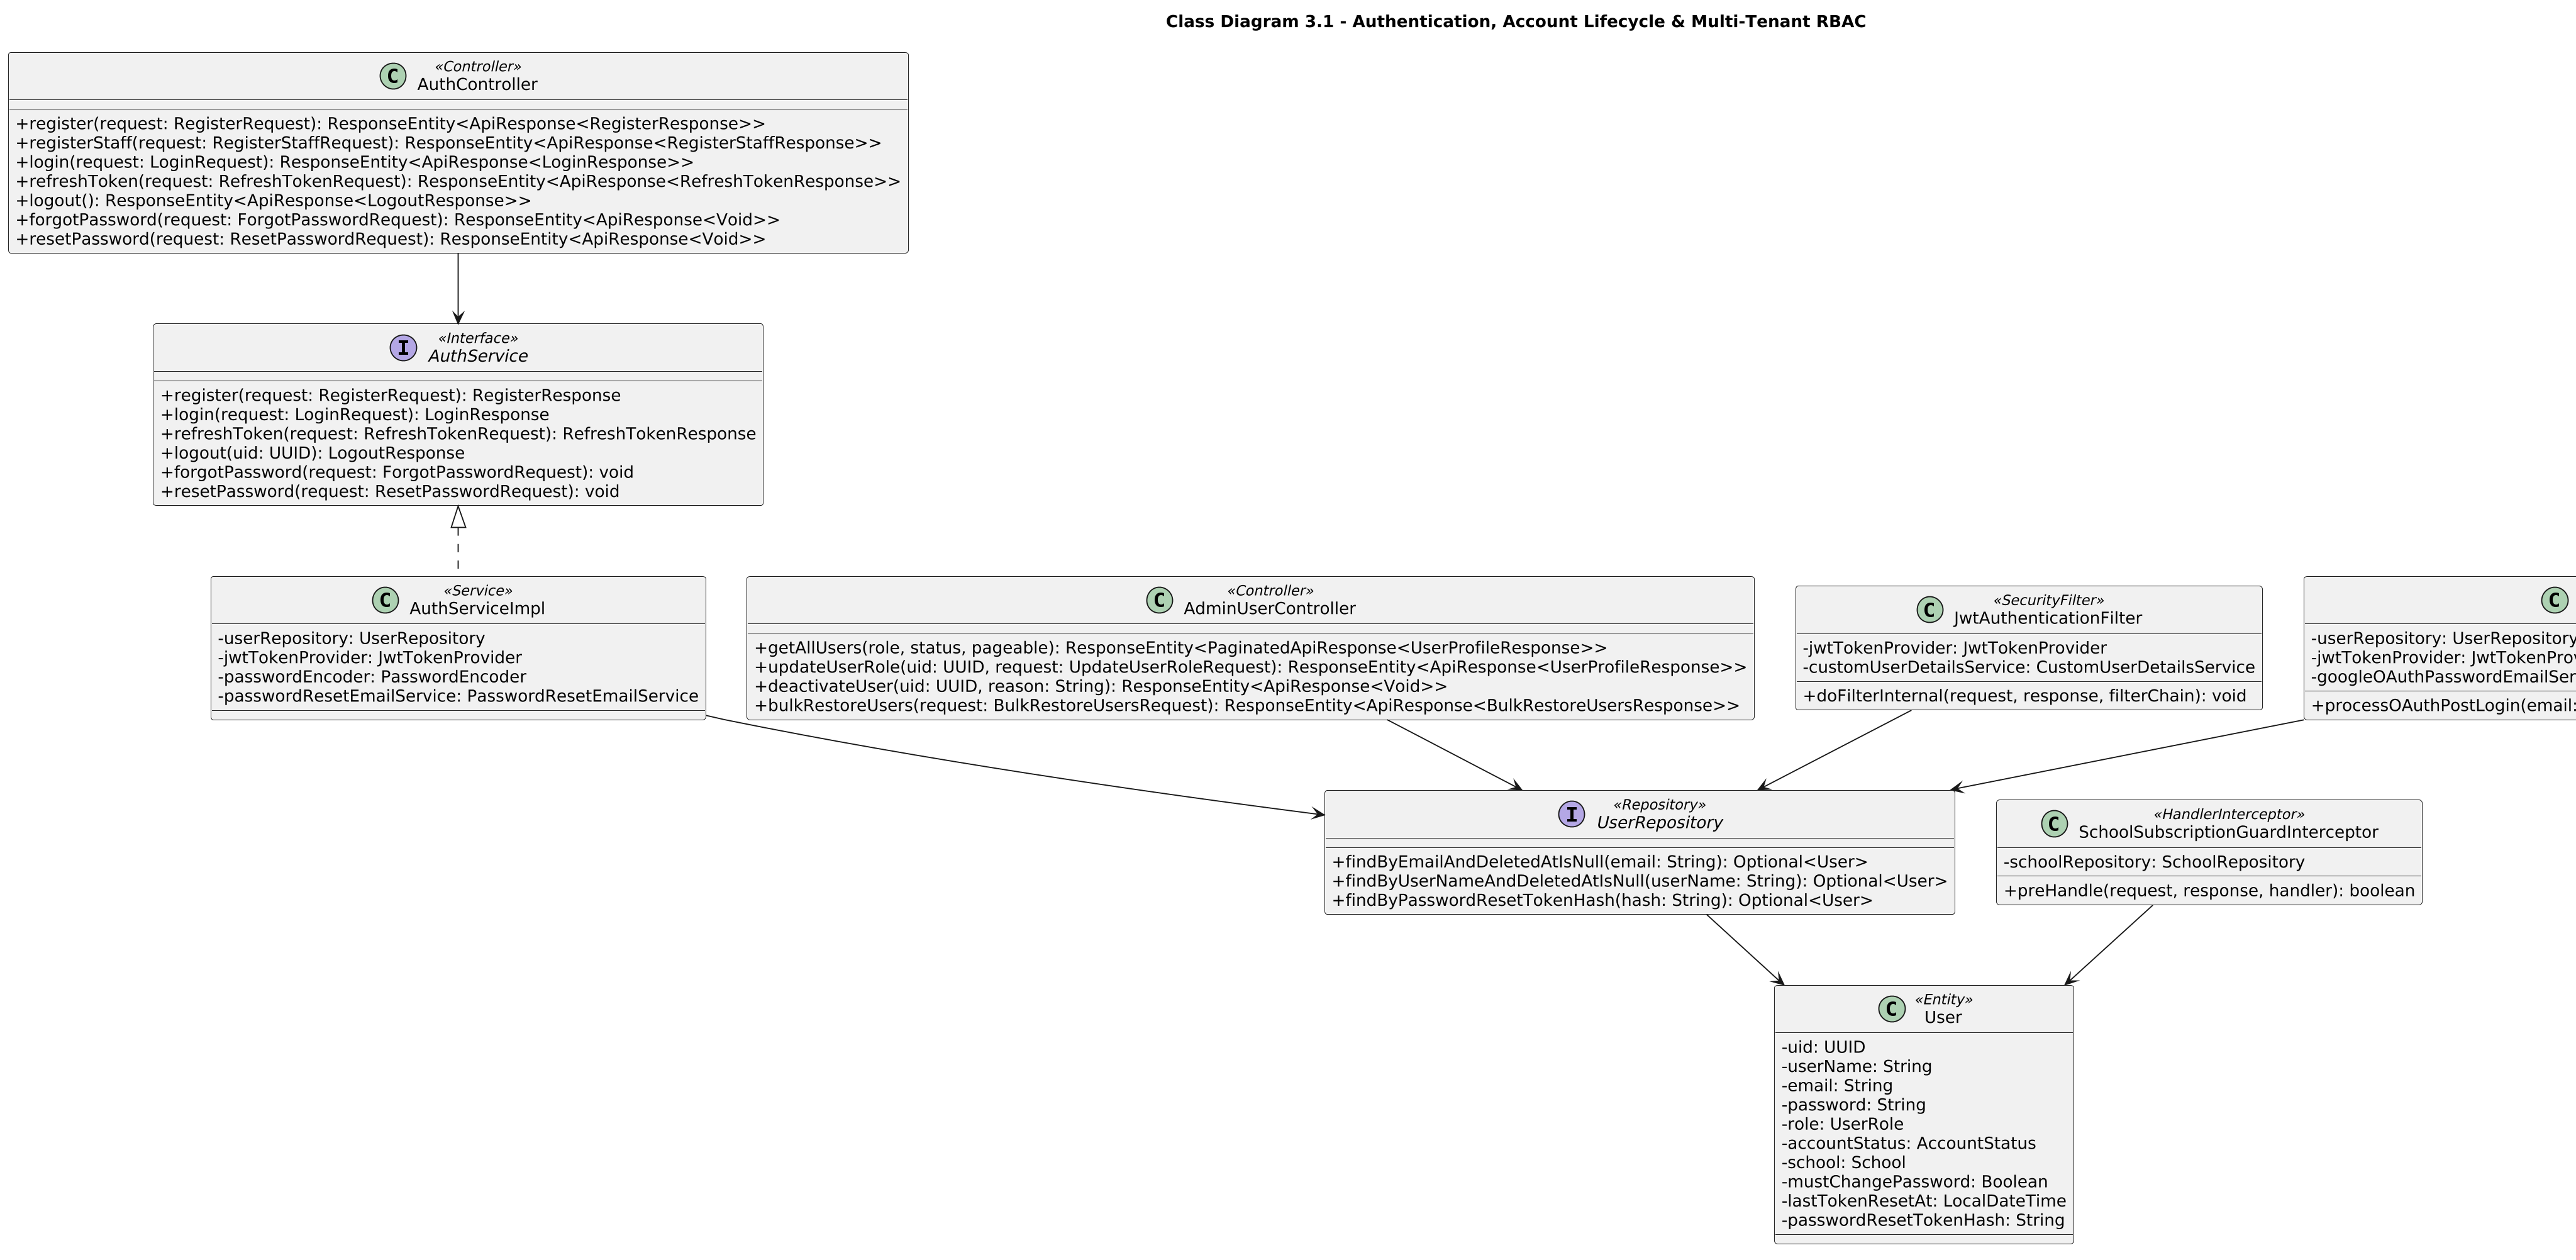
\includegraphics[width=0.98\textwidth]{figures/cls_01_auth_rbac.png}
    \caption{Class Diagram -- Authentication, Account Lifecycle \& Multi-Tenant RBAC}
    \label{fig:cls_01_auth_rbac}
\end{figure}

\begin{longtable}{|L{5.2cm}|L{10.3cm}|}
\hline
\rowcolor{tableheader}
\textbf{Class} & \textbf{Description} \\
\hline
\endhead
\texttt{AuthController} & REST API controller (\texttt{/api/v1/auth}) handling customer registration, staff registration, credential login, JWT refresh token rotation, logout, and forgot/reset password endpoints. \\
\hline
\texttt{AdminUserController} & REST API controller (\texttt{/api/v1/admin/users}) enabling \texttt{SYSTEM\_ADMIN} and \texttt{SCHOOL\_ADMIN} to query paginated user lists, update user roles, deactivate accounts, and bulk-restore soft-deleted users. \\
\hline
\texttt{UserController} & REST API controller (\texttt{/api/v1/users}) managing authenticated user profile retrieval, profile updates, and first-login mandatory password changes (\texttt{mustChangePassword}). \\
\hline
\texttt{JwtAuthenticationFilter} & Spring Security \texttt{OncePerRequestFilter} that extracts Bearer JWT tokens, validates signatures and \texttt{lastTokenResetAt} revocation timestamps, and populates \texttt{SecurityContextHolder}. \\
\hline
\texttt{SchoolSubscriptionGuardInterceptor} & Spring MVC \texttt{HandlerInterceptor} enforcing B2B tenant guards: blocks institutional requests when the user's \texttt{School} is \texttt{SUSPENDED}, \texttt{INACTIVE}, or outside its \texttt{01/09}--\texttt{31/05} subscription window. \\
\hline
\texttt{AuthService} / \texttt{AuthServiceImpl} & Core authentication service interface and implementation managing BCrypt password verification, dual-token issuance, token revocation via \texttt{lastTokenResetAt}, and SHA-256 hashed password reset tokens. \\
\hline
\texttt{GoogleOAuthServiceImpl} & Processes Google OAuth 2.0 SSO callbacks, auto-provisions first-time \texttt{CUSTOMER} accounts with random BCrypt passwords, and dispatches credentials via \texttt{GoogleOAuthPasswordEmailService}. \\
\hline
\texttt{JwtTokenProvider} & Cryptographic utility built on \texttt{jjwt 0.12.5} for signing and parsing access and refresh JWTs containing \texttt{uid}, \texttt{role}, and \texttt{schoolId} claims. \\
\hline
\texttt{UserRepository} & Spring Data JPA repository providing query methods for active/deleted users by email, username, school tenant, and password reset token hash. \\
\hline
\texttt{User} & Core JPA domain entity mapped to \texttt{"user"}, encapsulating identity, 6-role RBAC (\texttt{UserRole}), \texttt{AccountStatus}, B2C/B2B token counters, and audit timestamps. \\
\hline
\caption{Class Descriptions -- Authentication, Account Lifecycle \& Multi-Tenant RBAC}
\label{tab:cls_01_auth_rbac}
\end{longtable}

\subsubsection{Sequence Diagrams: Authentication \& Account Lifecycle}

\begin{figure}[H]
    \centering
    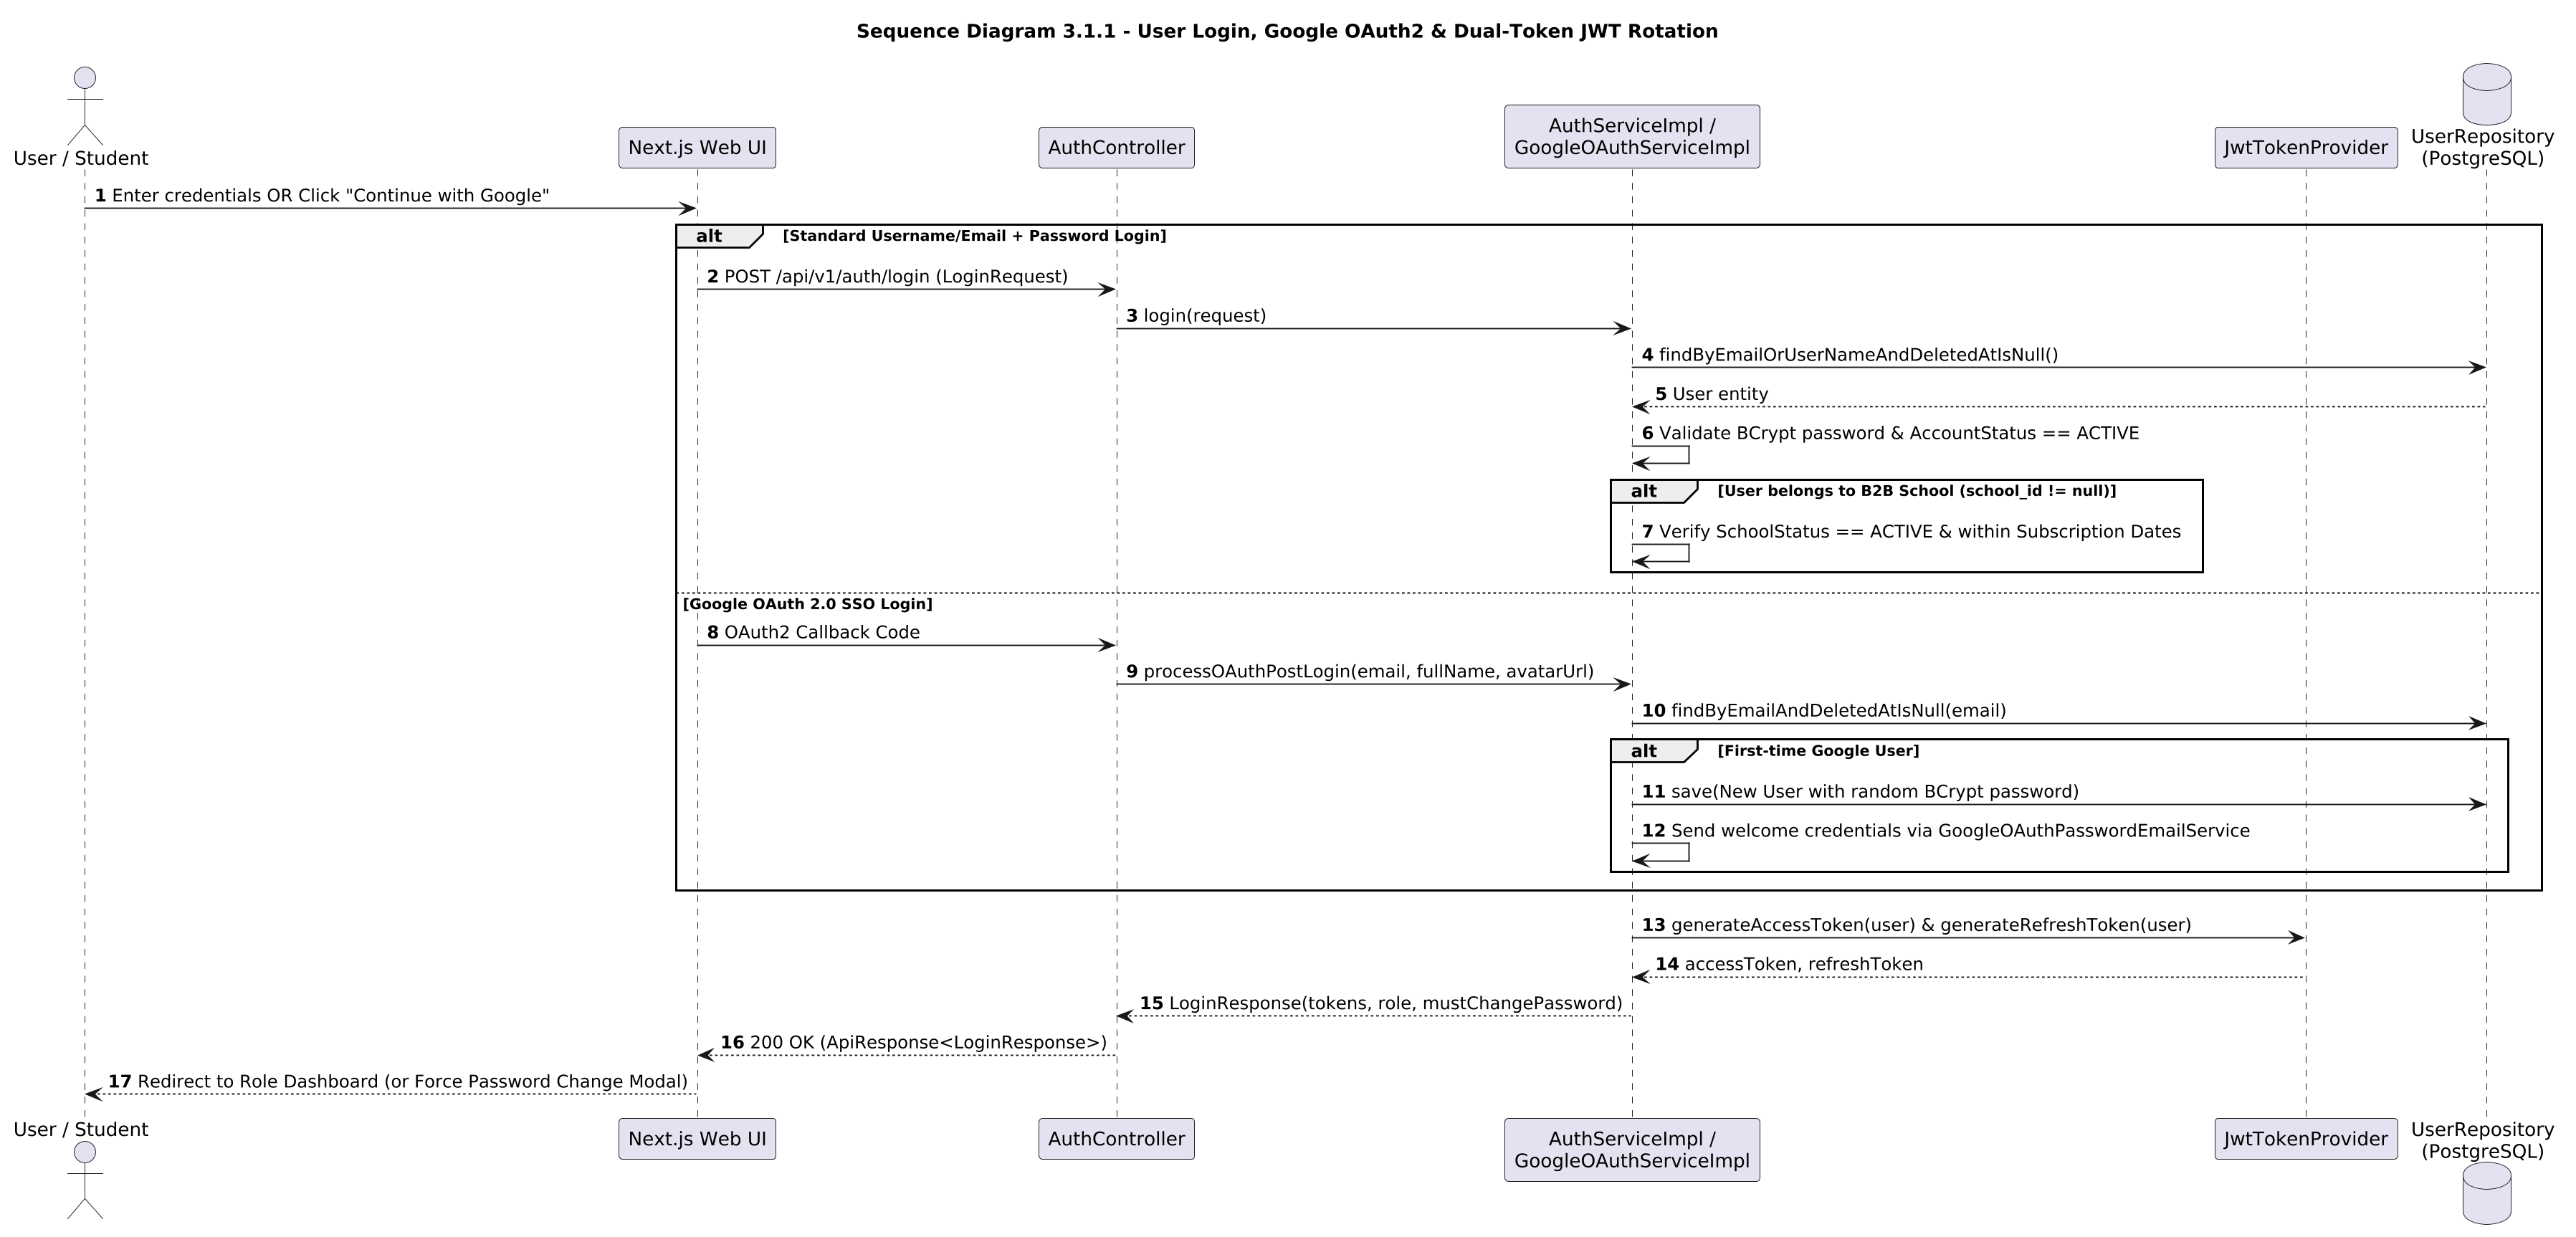
\includegraphics[width=0.98\textwidth]{figures/seq_01_login_oauth_jwt.png}
    \caption{Sequence Diagram -- User Login, Google OAuth2 \& Dual-Token JWT Rotation}
    \label{fig:seq_01_login_oauth_jwt}
\end{figure}

\begin{figure}[H]
    \centering
    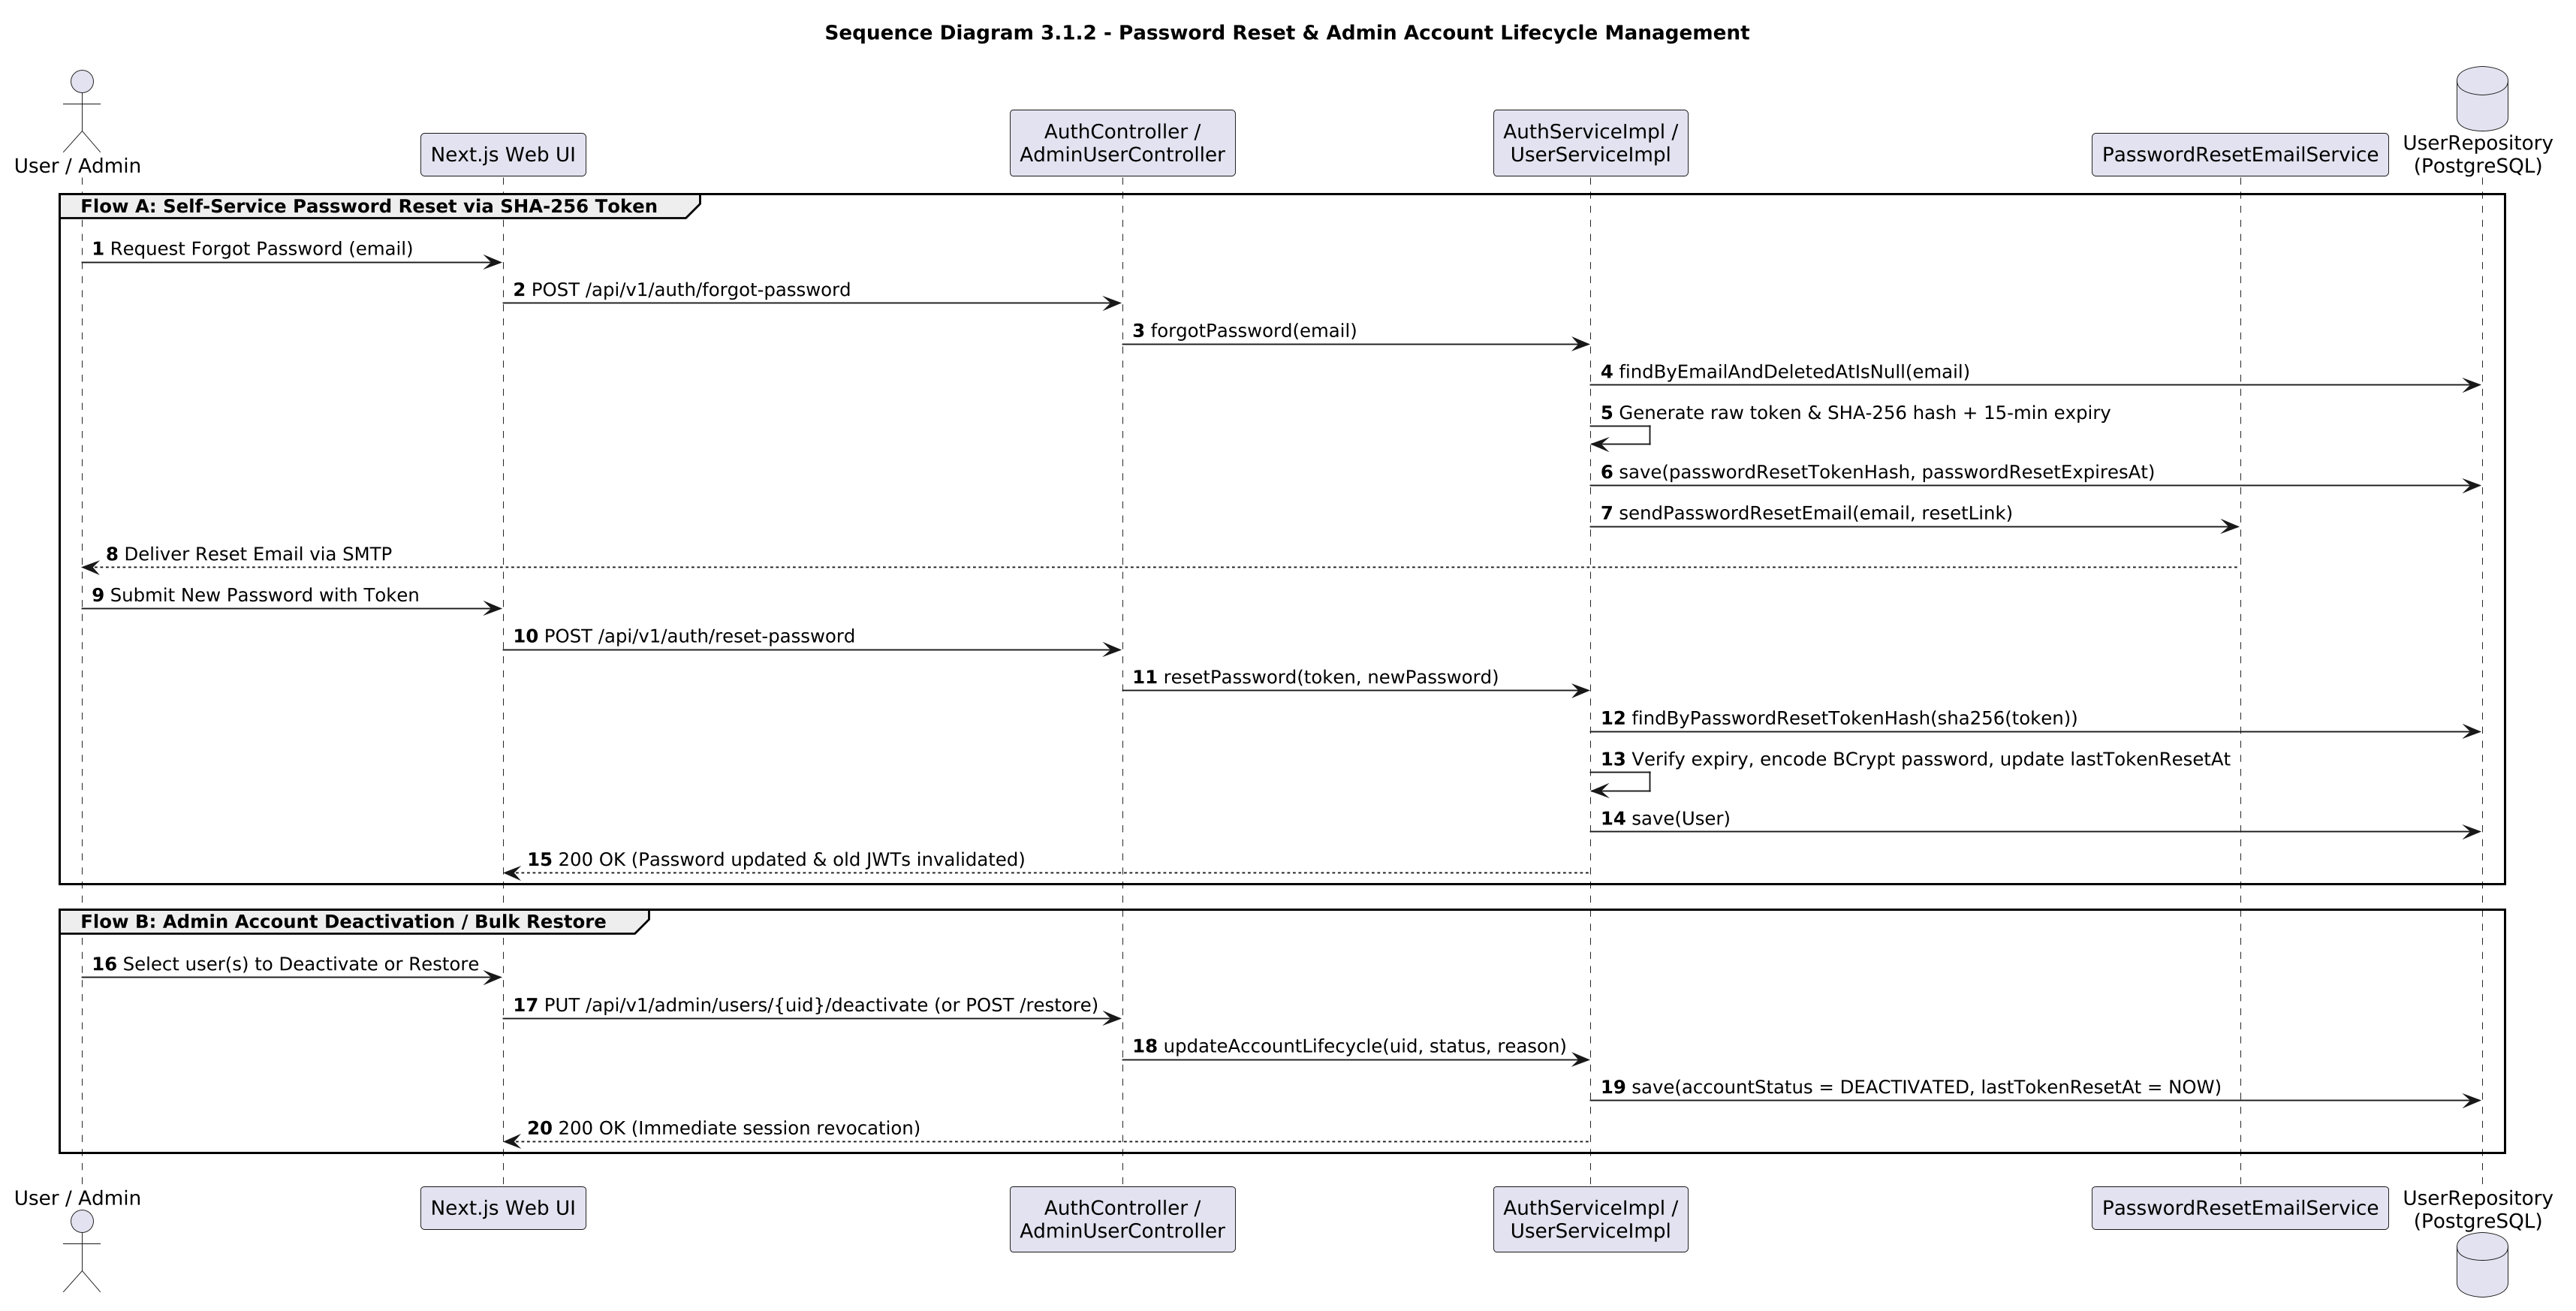
\includegraphics[width=0.98\textwidth]{figures/seq_02_password_reset_and_lifecycle.png}
    \caption{Sequence Diagram -- Self-Service Password Reset \& Admin Account Lifecycle Management}
    \label{fig:seq_02_password_reset_and_lifecycle}
\end{figure}

\newpage
\subsection{B2B SaaS School, Classroom \& Token Quota Allocation}

\subsubsection{Class Diagram: B2B SaaS School, Classroom \& Token Quota Allocation}

\begin{figure}[H]
    \centering
    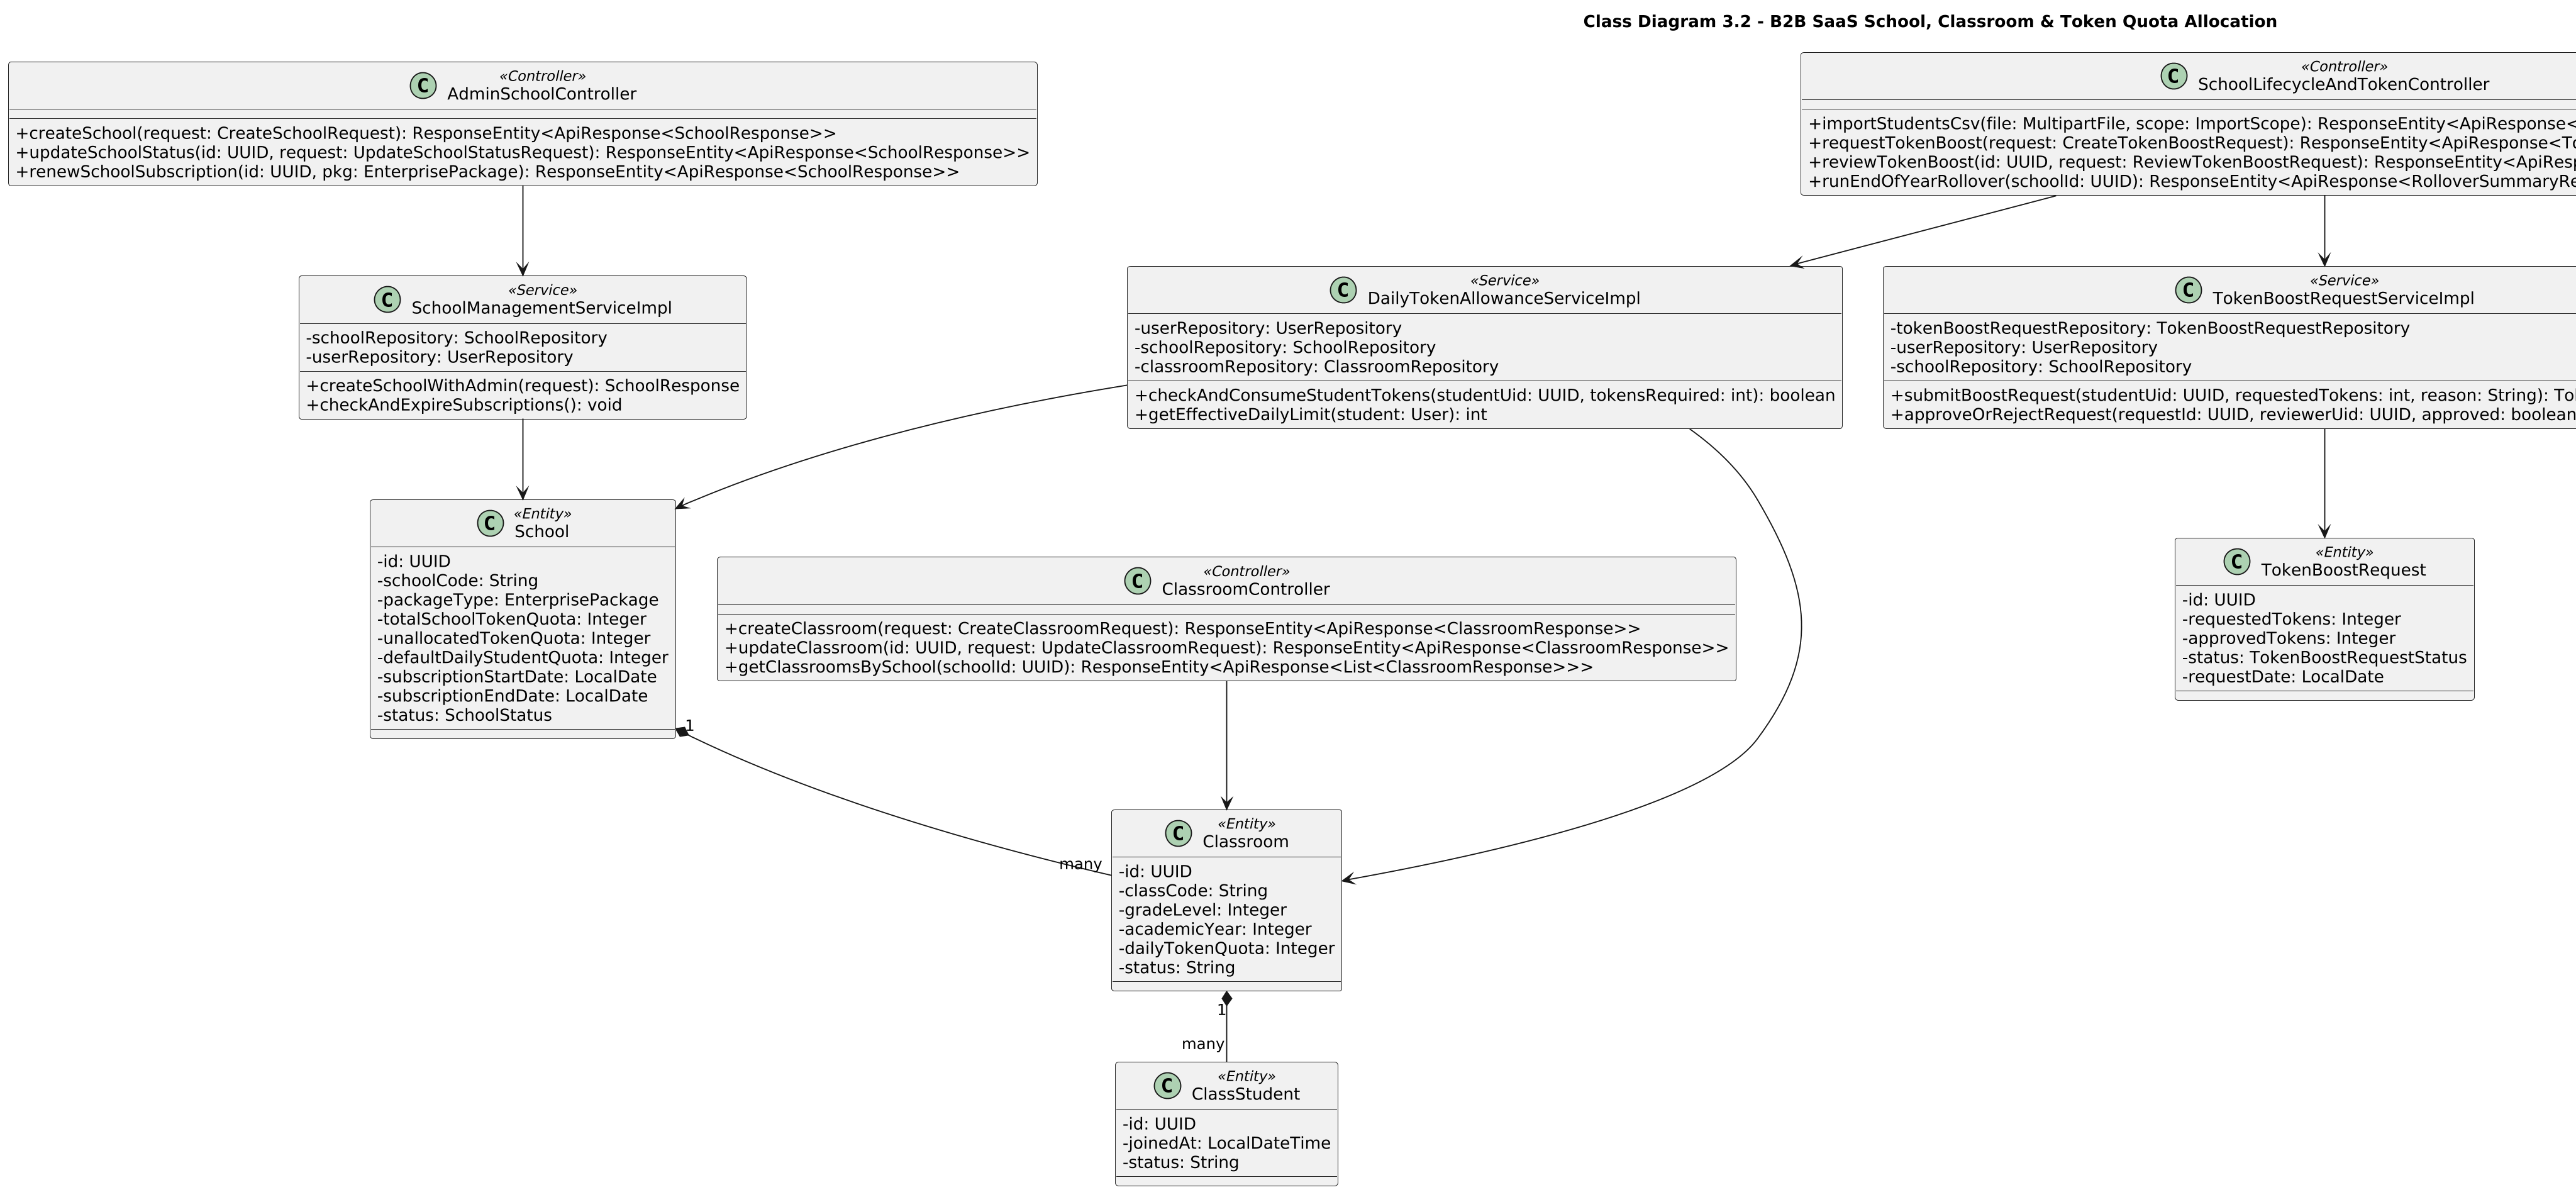
\includegraphics[width=0.98\textwidth]{figures/cls_02_school_classroom_token.png}
    \caption{Class Diagram -- B2B SaaS School, Classroom \& Token Quota Allocation}
    \label{fig:cls_02_school_classroom_token}
\end{figure}

\begin{longtable}{|L{5.5cm}|L{10.0cm}|}
\hline
\rowcolor{tableheader}
\textbf{Class} & \textbf{Description} \\
\hline
\endhead
\texttt{AdminSchoolController} & REST API controller (\texttt{/api/v1/admin/schools}) for \texttt{SYSTEM\_ADMIN} to provision B2B school tenants, assign \texttt{EnterprisePackage} tiers, and manage school subscription statuses. \\
\hline
\texttt{ClassroomController} / \texttt{ClassroomStudentController} & REST API controllers managing school classrooms, teacher assignments, student roster listings, classroom transfers, and smart class join codes (\texttt{SmartClassCodeGenerator}). \\
\hline
\texttt{SchoolLifecycleAndTokenController} & REST API controller (\texttt{/api/v1/schools}) handling bulk CSV student imports, daily token boost requests/approvals, and end-of-academic-year student lifecycle rollovers. \\
\hline
\texttt{SchoolManagementServiceImpl} & Manages school creation, initial \texttt{SCHOOL\_ADMIN} provisioning, enterprise token pool initialization, and scheduled subscription expiration checks. \\
\hline
\texttt{AcademicLifecycleServiceImpl} & Executes end-of-year academic promotions: promotes Grade 6--11 classrooms, archives completed cohorts, and transitions graduating Grade 12 student accounts to \texttt{DEACTIVATED}. \\
\hline
\texttt{StudentImportServiceImpl} & Coordinates \texttt{SchoolWideImportProcessor} and \texttt{ClassroomImportProcessor} using \texttt{Apache Commons CSV} to batch-create student accounts and auto-exempt past-deadline classroom assignments. \\
\hline
\texttt{DailyTokenAllowanceServiceImpl} & Enforces B2B student daily token limits with lazy midnight resets, resolving effective limits from classroom overrides or school defaults plus approved daily bonus tokens. \\
\hline
\texttt{TokenBoostRequestServiceImpl} & Manages the student daily token boost lifecycle (\texttt{PENDING} $\rightarrow$ \texttt{APPROVED}/\texttt{REJECTED}), deducting approved tokens from the school's shared \texttt{unallocatedTokenQuota}. \\
\hline
\texttt{School}, \texttt{Classroom}, \texttt{ClassStudent}, \texttt{TokenBoostRequest} & Persistent JPA domain entities modeling the multi-tenant school hierarchy, classroom rosters, and daily token boost requests. \\
\hline
\caption{Class Descriptions -- B2B SaaS School, Classroom \& Token Quota Allocation}
\label{tab:cls_02_school_classroom_token}
\end{longtable}

\subsubsection{Sequence Diagrams: School Provisioning, CSV Import \& Token Boost}

\begin{figure}[H]
    \centering
    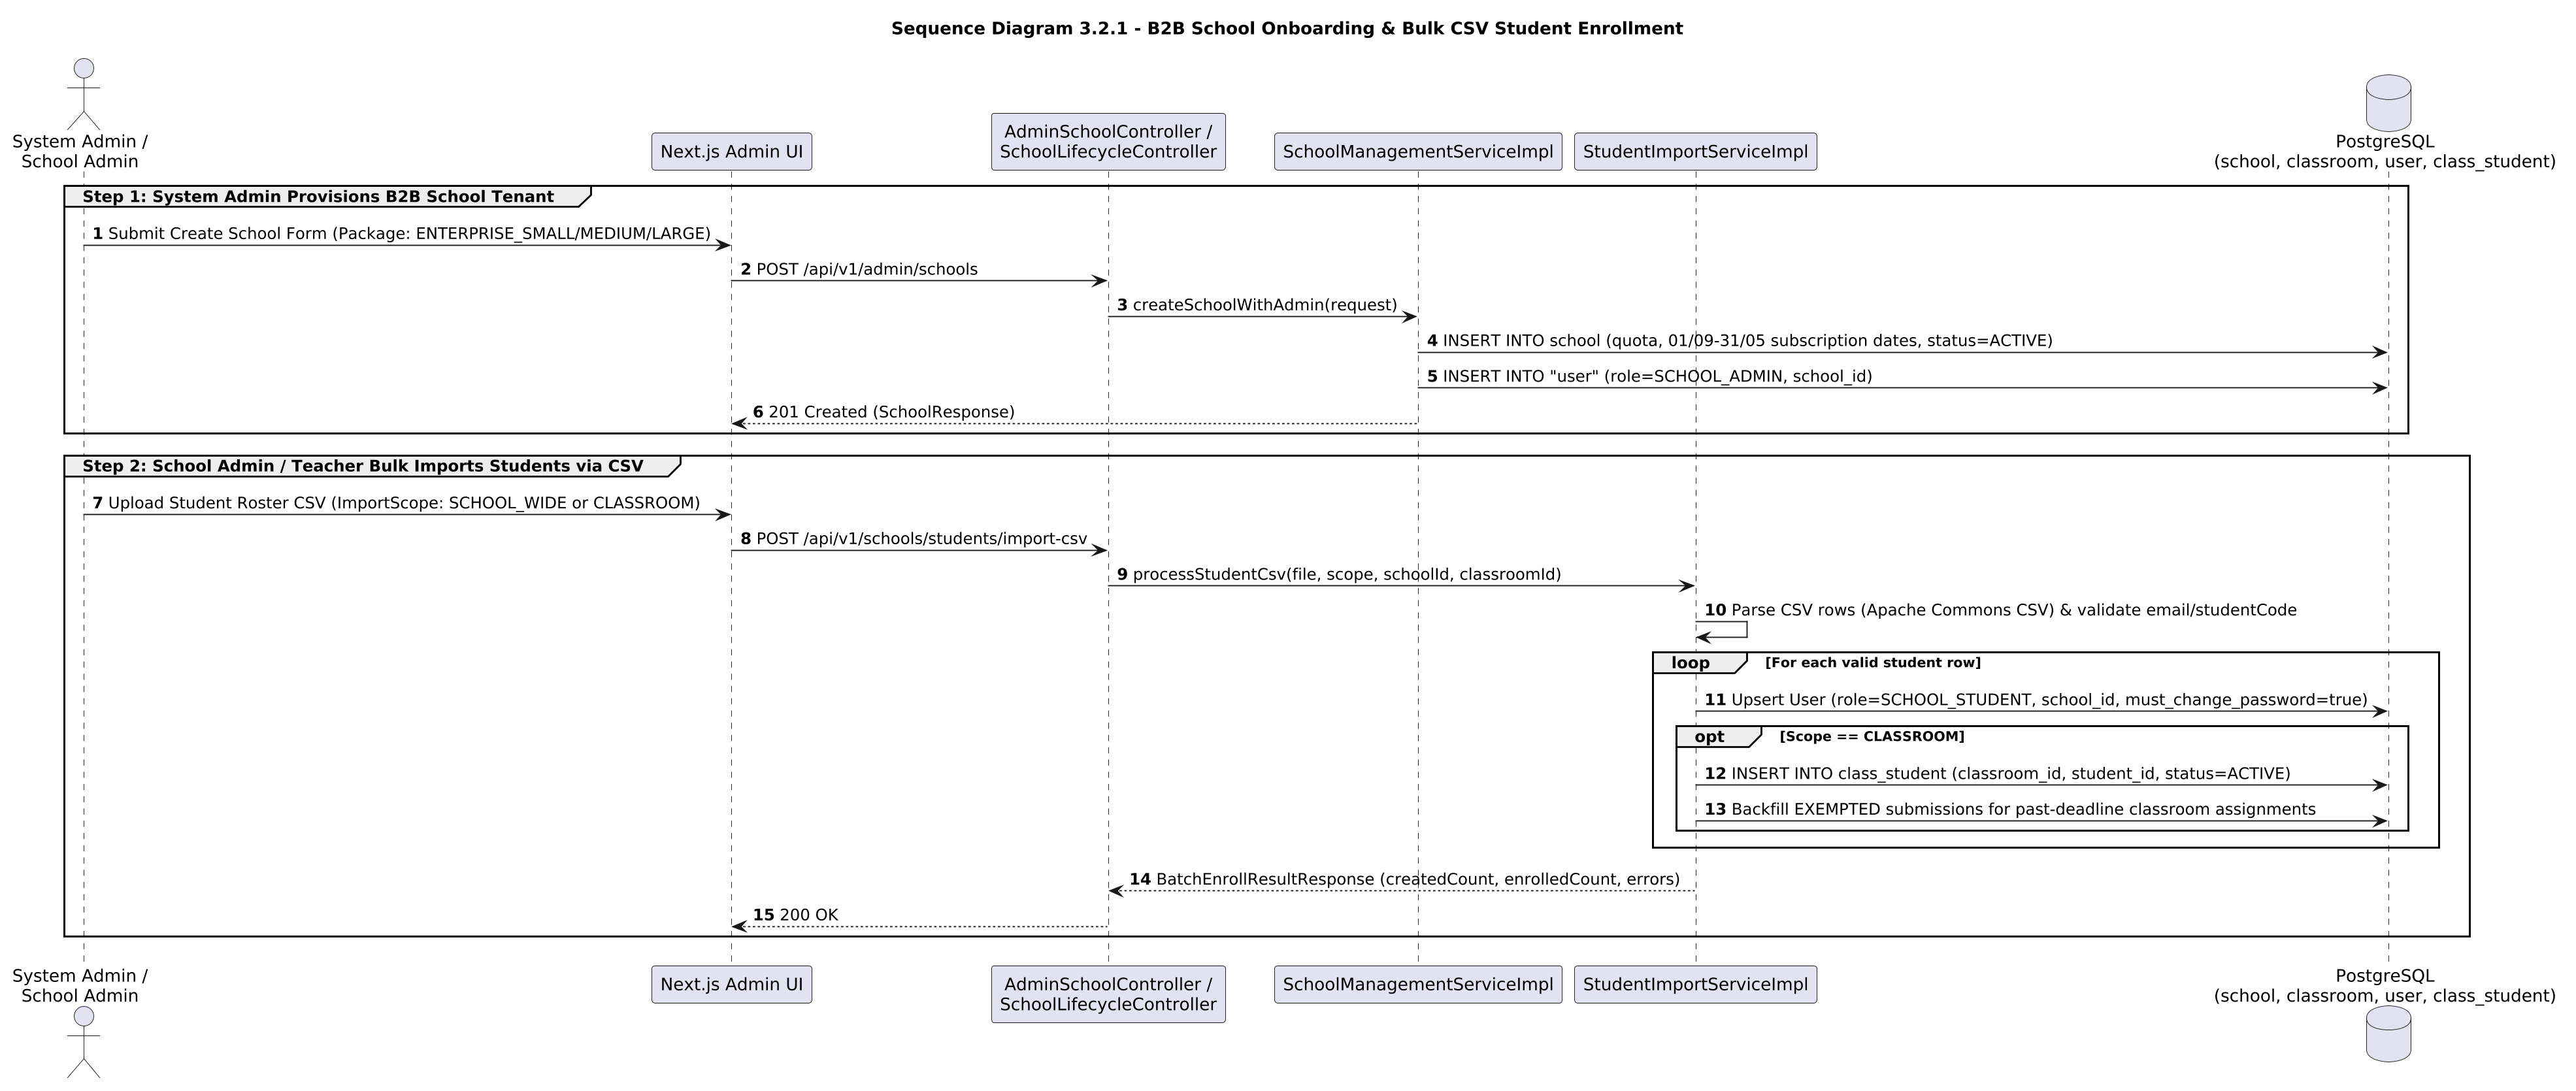
\includegraphics[width=0.98\textwidth]{figures/seq_03_school_provisioning_and_import.png}
    \caption{Sequence Diagram -- B2B School Onboarding \& Bulk CSV Student Enrollment}
    \label{fig:seq_03_school_provisioning_and_import}
\end{figure}

\begin{figure}[H]
    \centering
    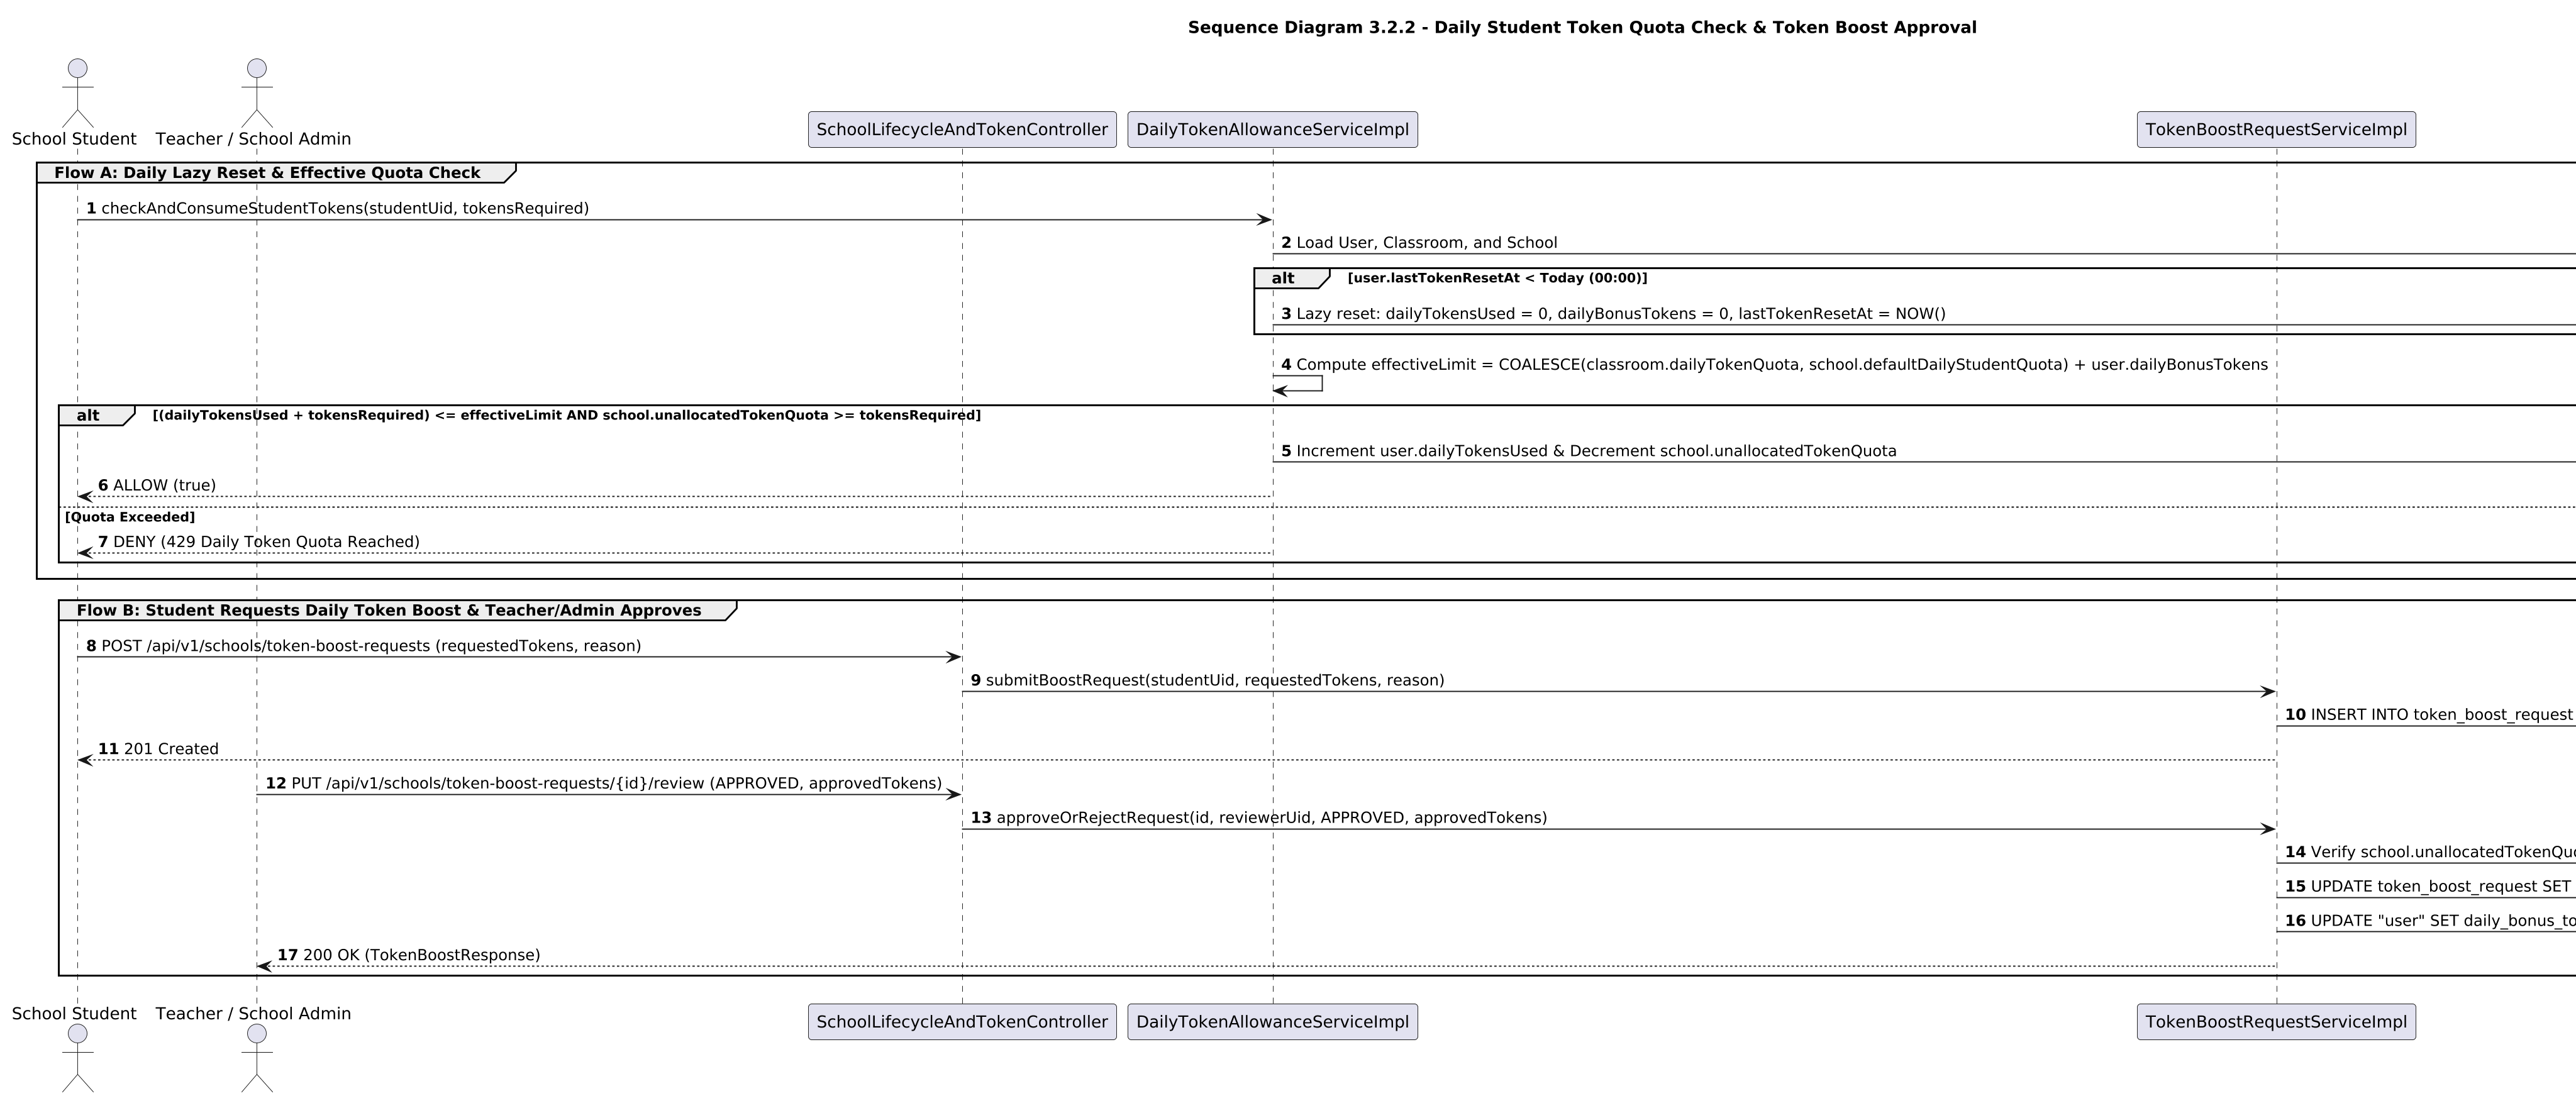
\includegraphics[width=0.98\textwidth]{figures/seq_04_token_boost_and_allowance.png}
    \caption{Sequence Diagram -- Daily Student Token Quota Check \& Token Boost Request Approval}
    \label{fig:seq_04_token_boost_and_allowance}
\end{figure}

\newpage
\subsection{Historical Content, Character, Document OCR \& Interactive Map}

\subsubsection{Class Diagram: Historical Content, Character, Document OCR \& Interactive Map}

\begin{figure}[H]
    \centering
    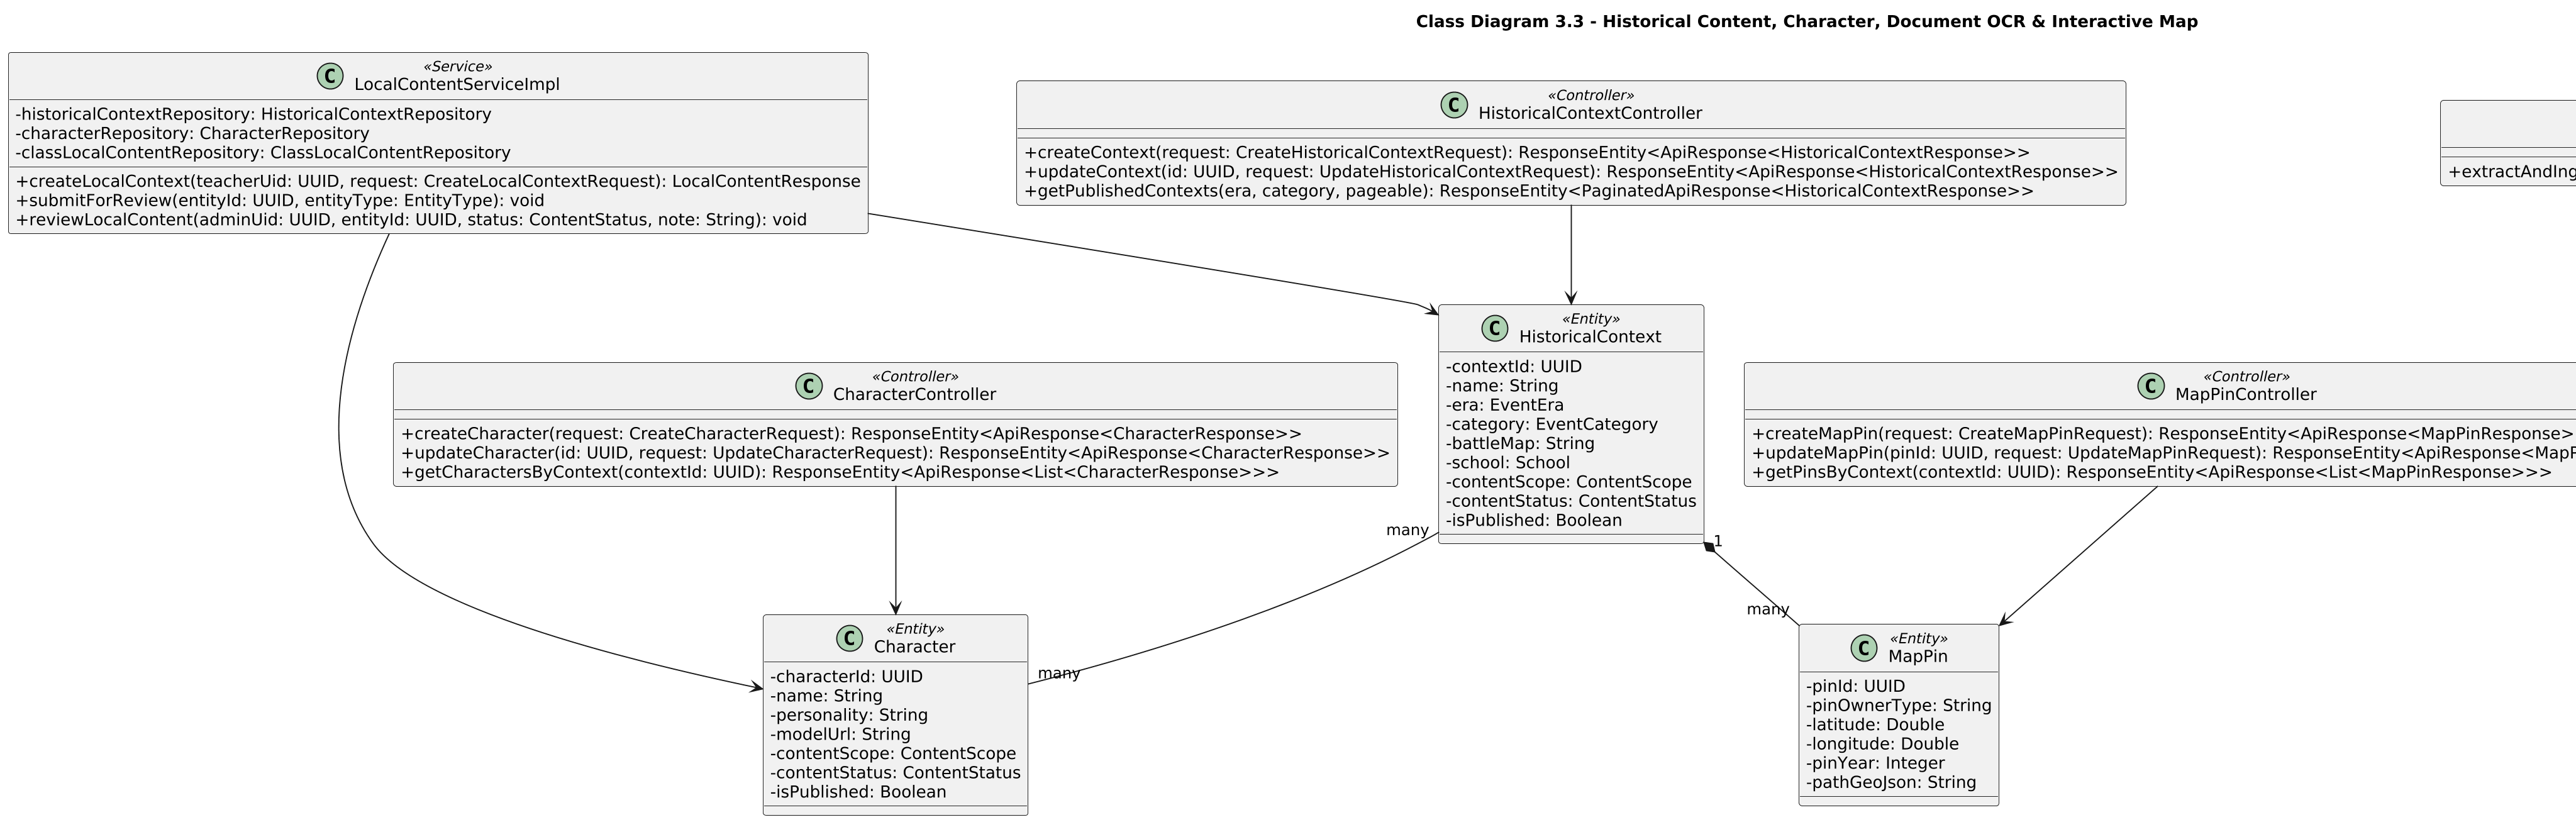
\includegraphics[width=0.98\textwidth]{figures/cls_03_content_character_map.png}
    \caption{Class Diagram -- Historical Content, Character, Document OCR \& Interactive Map}
    \label{fig:cls_03_content_character_map}
\end{figure}

\begin{longtable}{|L{5.5cm}|L{10.0cm}|}
\hline
\rowcolor{tableheader}
\textbf{Class} & \textbf{Description} \\
\hline
\endhead
\texttt{HistoricalContextController} & REST API controller (\texttt{/api/v1/historical-contexts}) providing CRUD, publication toggling, and filtered timeline pagination by \texttt{EventEra} and \texttt{EventCategory}. \\
\hline
\texttt{CharacterController} & REST API controller (\texttt{/api/v1/characters}) managing historical character biographies, persona prompts, 3D model URLs, and context associations. \\
\hline
\texttt{PdfExtractionController} / \texttt{DocumentFileController} & REST API controllers handling PDF upload, automatic text/OCR extraction, document persistence, and asynchronous RAG vector indexing triggers. \\
\hline
\texttt{MapPinController} / \texttt{MapFocusController} & REST API controllers managing GeoJSON battle-map pins (\texttt{ADMIN} and \texttt{USER} pins), troop movement \texttt{LineString} paths, and camera viewpoint focuses. \\
\hline
\texttt{TeacherLocalContentController} / \texttt{SchoolAdminLocalContentController} & REST API controllers enabling teachers to author local history contexts/characters and school admins to review and approve/reject them (\texttt{PENDING\_REVIEW} $\rightarrow$ \texttt{ACTIVE}/\texttt{DRAFT}). \\
\hline
\texttt{PdfExtractionServiceImpl} / \texttt{OcrServiceImpl} & Classifies uploaded PDFs via \texttt{PdfTypeClassifier}; extracts digital text via \texttt{Apache PDFBox 3.0.1} or falls back to \texttt{Tess4J 5.10.0} Vietnamese OCR (\texttt{vie.traineddata}) for scanned historical archives. \\
\hline
\texttt{LocalContentServiceImpl} & Enforces multi-tenant isolation and policy checks (\texttt{localHistoryPolicyAccepted}) for school-owned local historical content and classroom assignments (\texttt{ClassLocalContent}). \\
\hline
\texttt{HistoricalContext}, \texttt{Character}, \texttt{Document}, \texttt{MapPin}, \texttt{MapFocus} & Domain entities representing historical events, roleplay personas, RAG source documents, and interactive GeoJSON map elements. \\
\hline
\caption{Class Descriptions -- Historical Content, Character, Document OCR \& Interactive Map}
\label{tab:cls_03_content_character_map}
\end{longtable}

\subsubsection{Sequence Diagrams: PDF OCR Ingestion \& Local Content Approval}

\begin{figure}[H]
    \centering
    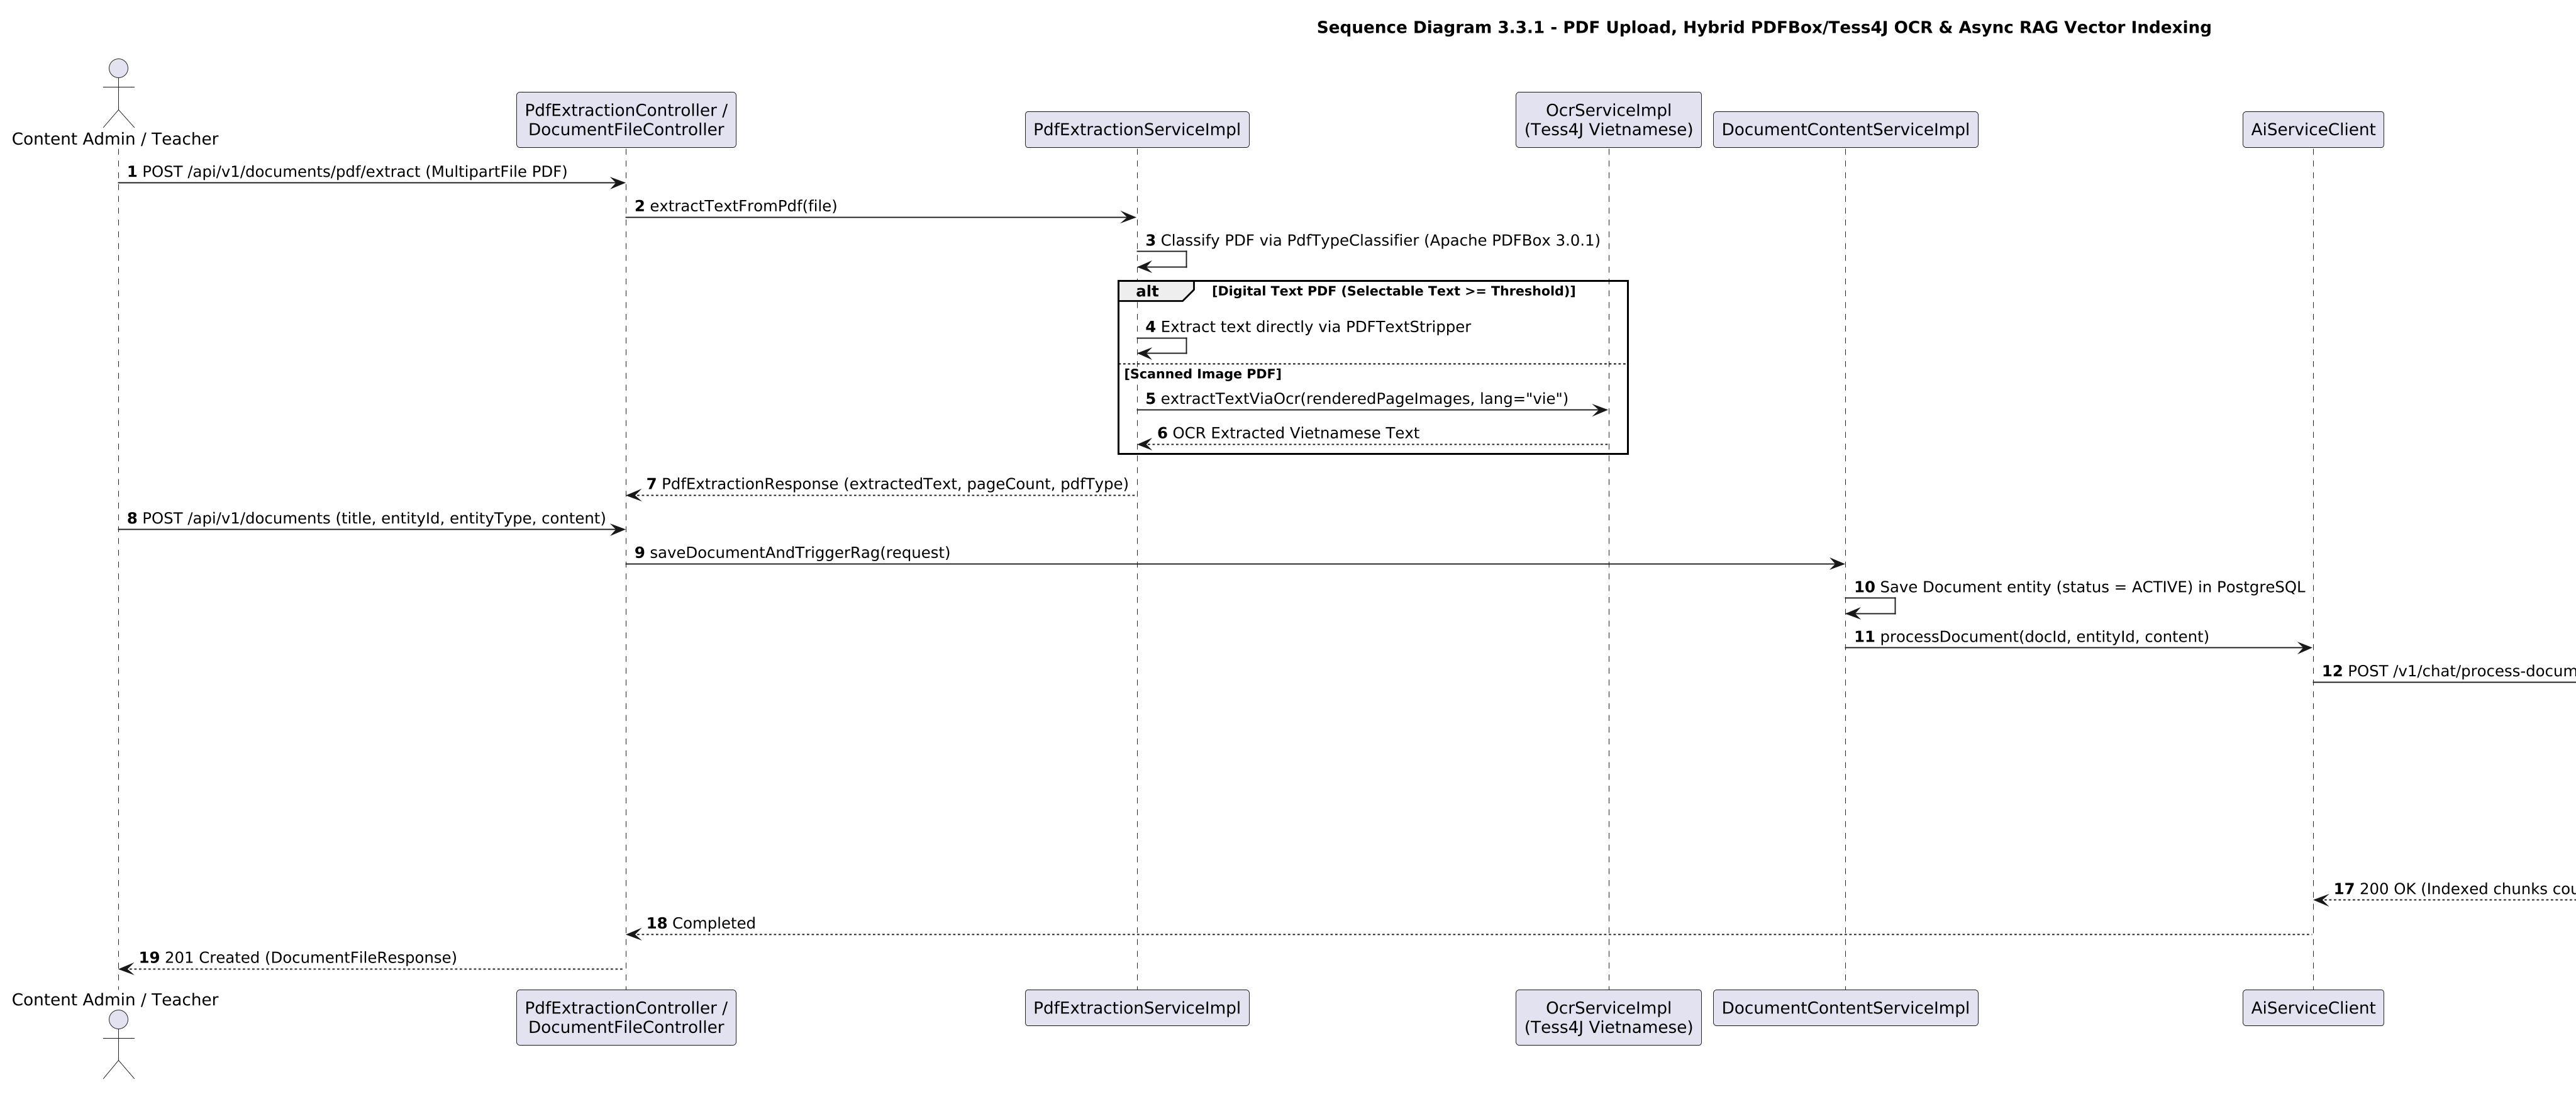
\includegraphics[width=0.98\textwidth]{figures/seq_05_document_ocr_and_rag_sync.png}
    \caption{Sequence Diagram -- PDF Upload, Hybrid PDFBox/Tess4J OCR \& Async RAG Vector Indexing}
    \label{fig:seq_05_document_ocr_and_rag_sync}
\end{figure}

\begin{figure}[H]
    \centering
    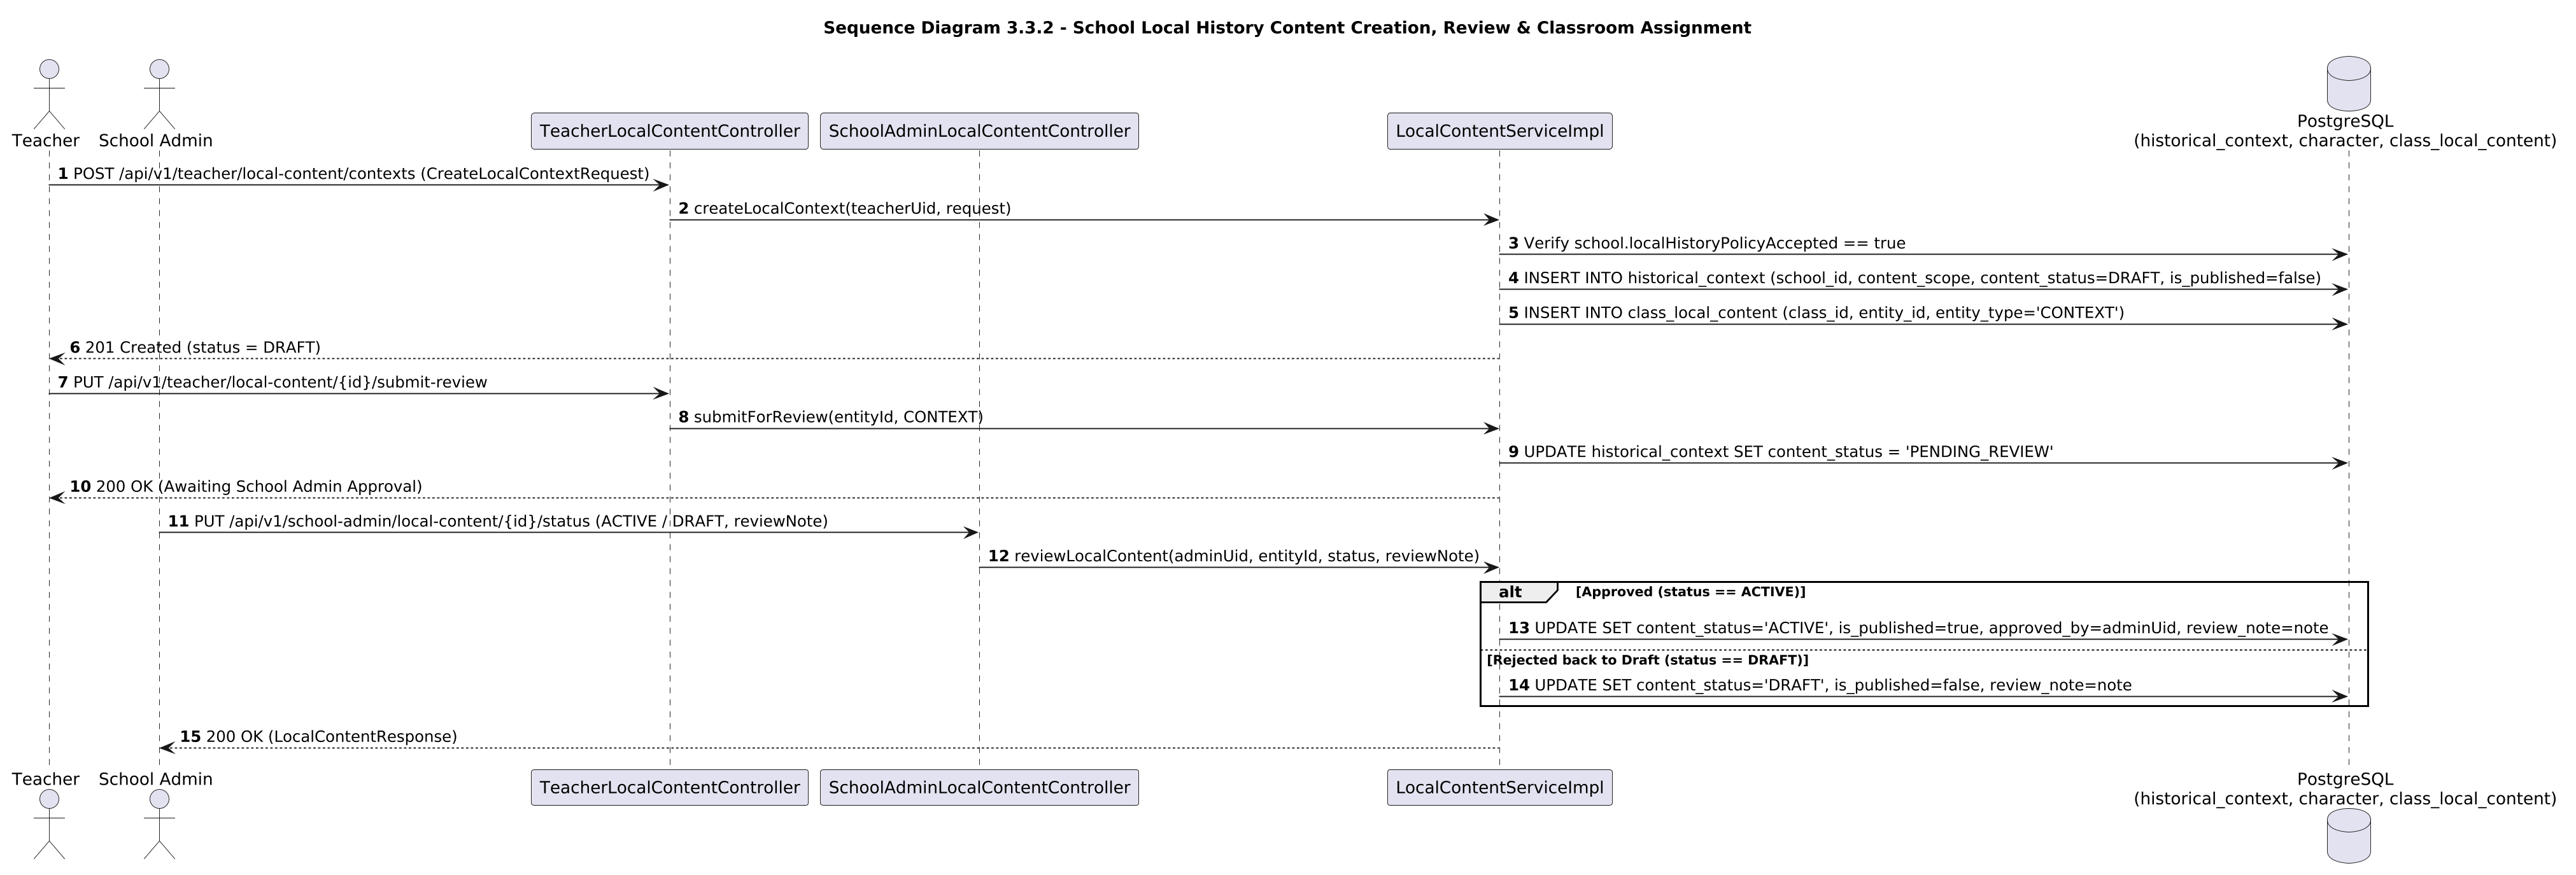
\includegraphics[width=0.98\textwidth]{figures/seq_06_local_content_approval.png}
    \caption{Sequence Diagram -- School Local History Content Creation, Review \& Classroom Assignment}
    \label{fig:seq_06_local_content_approval}
\end{figure}

\newpage
\subsection{Conversational AI Roleplay \& Hybrid RAG Microservice}

\subsubsection{Class Diagram: Conversational AI Roleplay \& Hybrid RAG Microservice}

\begin{figure}[H]
    \centering
    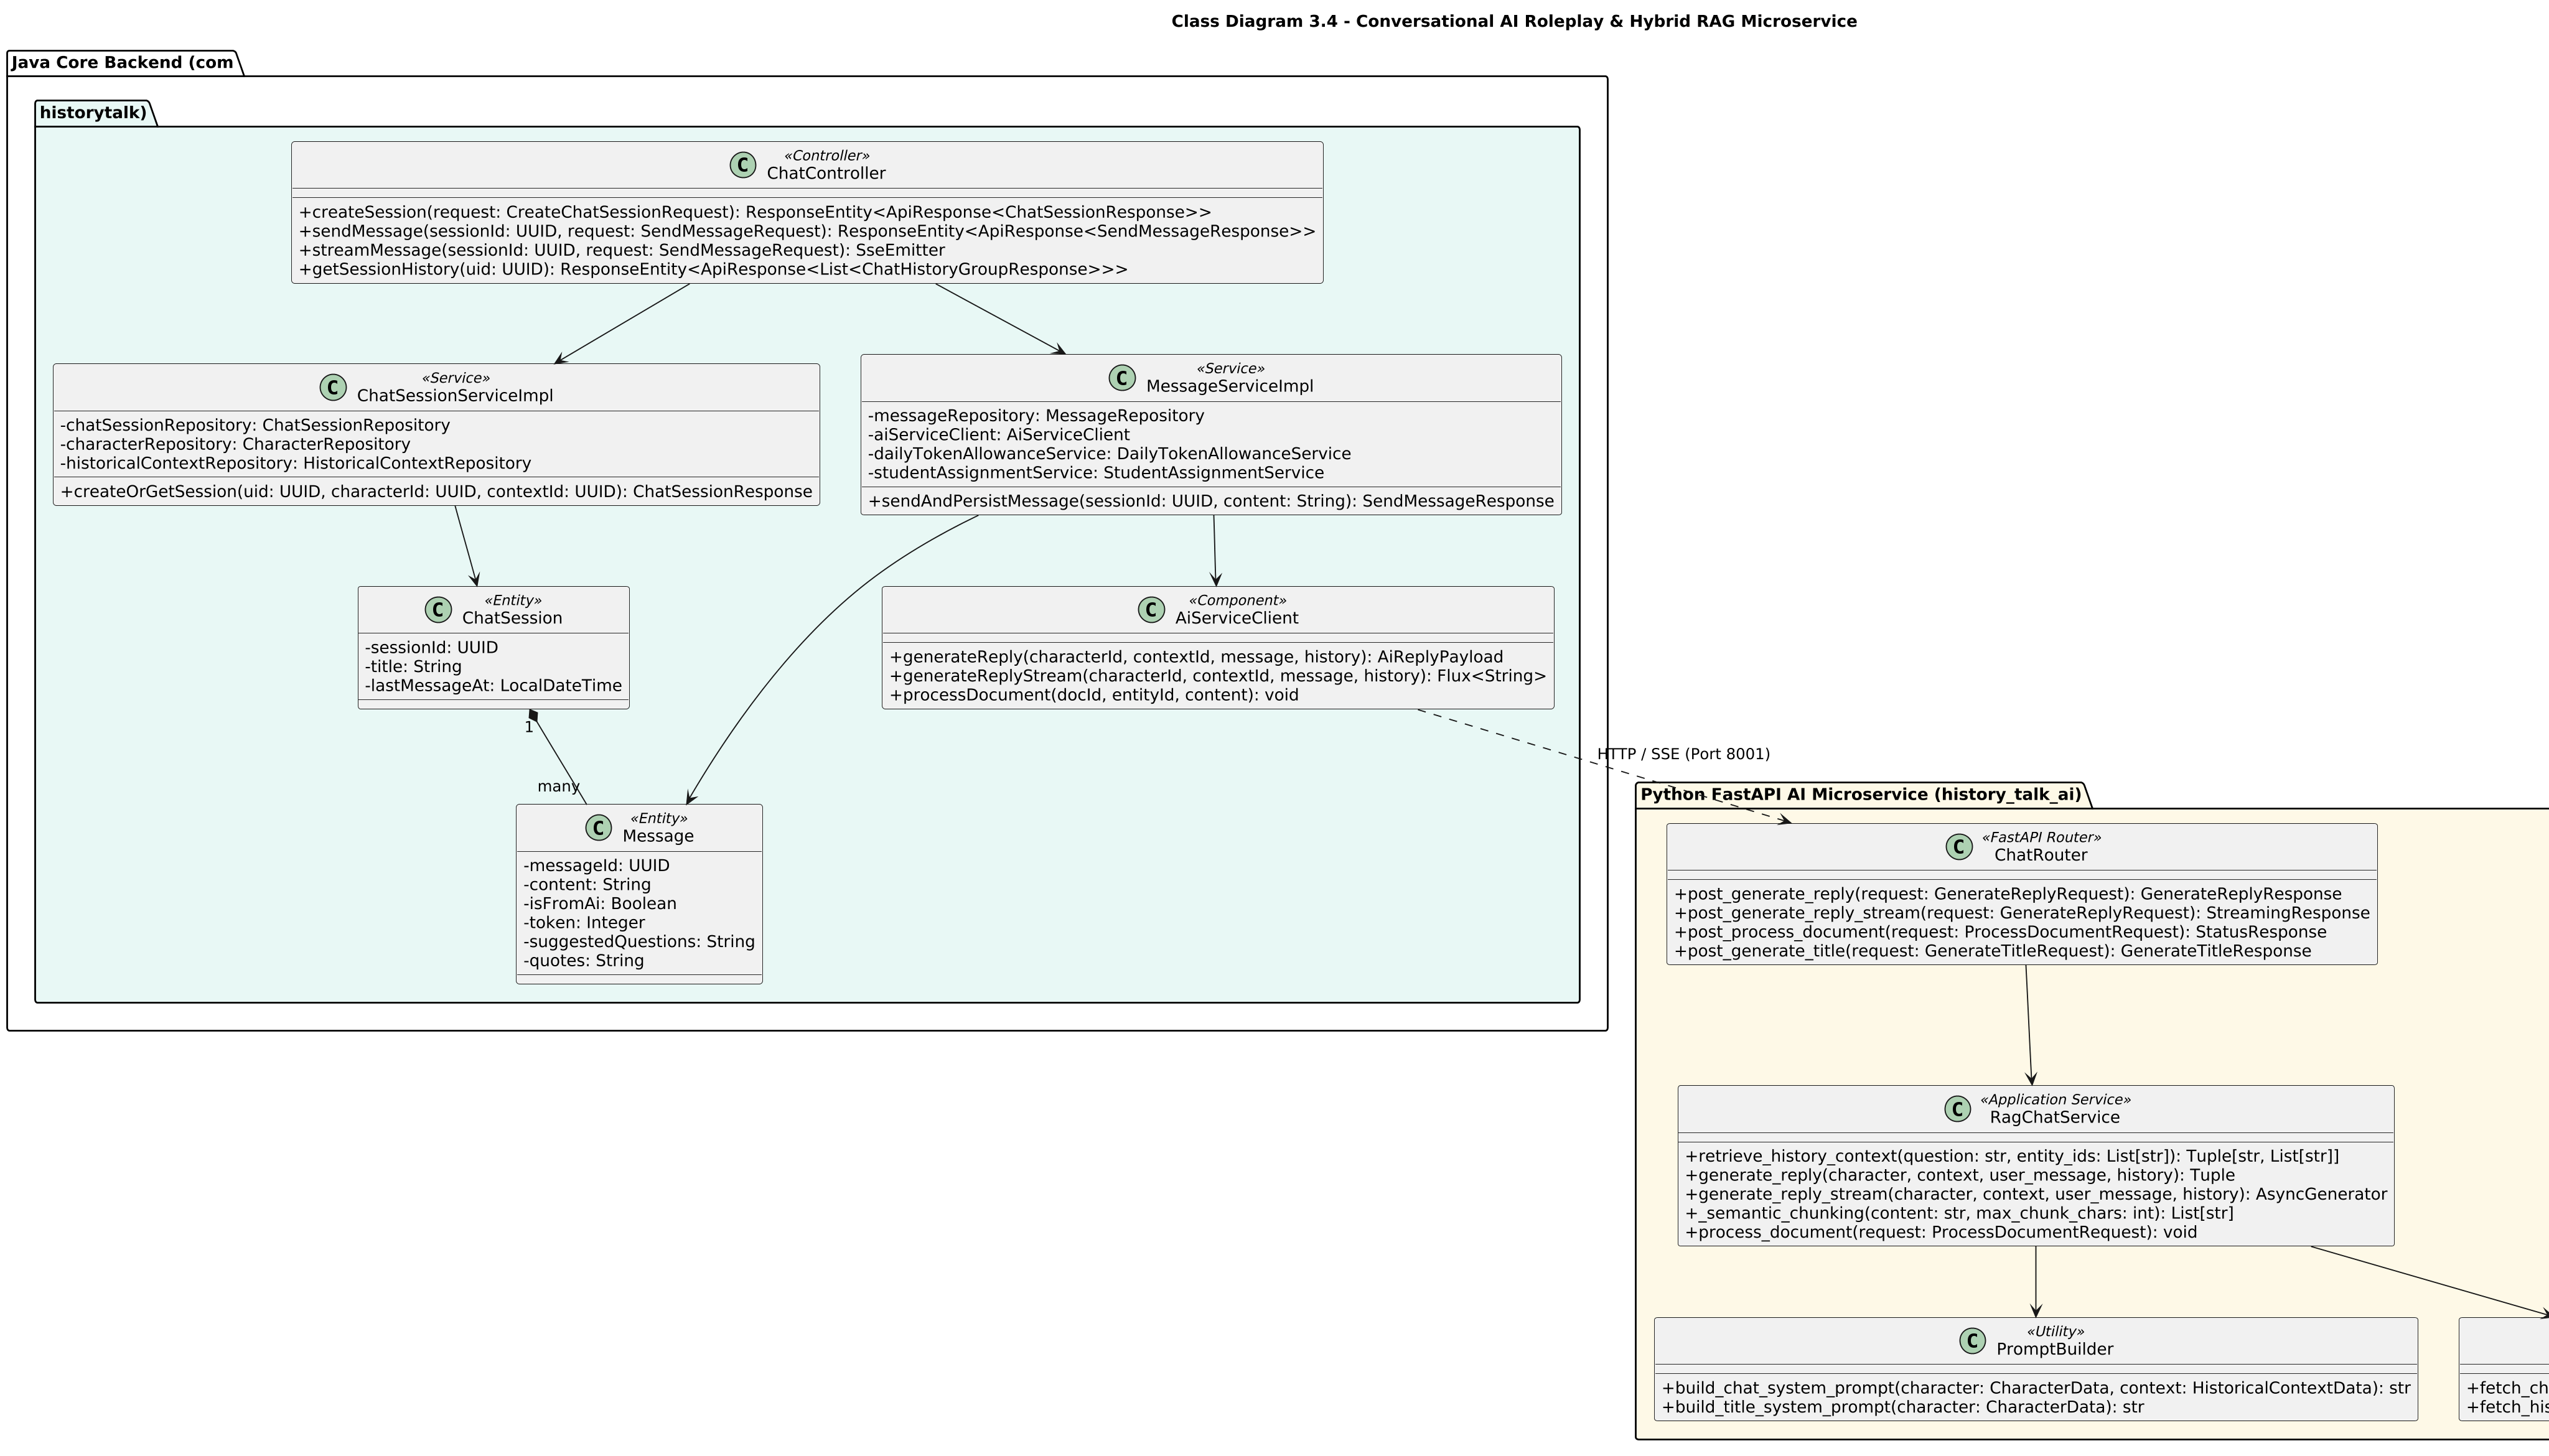
\includegraphics[width=0.98\textwidth]{figures/cls_04_chat_and_ai_rag.png}
    \caption{Class Diagram -- Conversational AI Roleplay \& Hybrid RAG Microservice}
    \label{fig:cls_04_chat_and_ai_rag}
\end{figure}

\begin{longtable}{|L{5.5cm}|L{10.0cm}|}
\hline
\rowcolor{tableheader}
\textbf{Class} & \textbf{Description} \\
\hline
\endhead
\texttt{ChatController} (Java) & Exposes endpoints (\texttt{/api/v1/chat}) for creating chat sessions, retrieving grouped conversation history, and streaming AI character responses over SSE. \\
\hline
\texttt{ChatSessionServiceImpl} (Java) & Manages chat session lifecycles, initial character greeting generation, and automatic short session title updates after the first dialogue exchange. \\
\hline
\texttt{MessageServiceImpl} (Java) & Coordinates token quota verification, user message persistence, AI microservice invocation, AI message persistence, and automatic \texttt{AI\_CHAT\_ROLEPLAY} assignment progress tracking. \\
\hline
\texttt{AiServiceClient} (Java) & HTTP/SSE integration client communicating with the Python FastAPI microservice using \texttt{X-Internal-Api-Key} authentication and Micrometer latency metrics (\texttt{AiMetricsService}). \\
\hline
\texttt{ChatRouter} (Python FastAPI) & Presentation router (\texttt{presentation/chat/router.py}) exposing \texttt{/v1/chat/generate-reply}, \texttt{/generate-reply-stream}, \texttt{/generate-title}, and \texttt{/process-document}. \\
\hline
\texttt{RagChatService} (Python FastAPI) & Core RAG module (\texttt{application/chat/service.py}) implementing dynamic 80th-percentile semantic chunking, \texttt{bge-m3} embedding generation, Supabase \texttt{match\_history\_chunks} RPC retrieval, Kaggle cross-encoder reranking, and streaming LLM roleplay. \\
\hline
\texttt{PromptBuilder} (Python FastAPI) & Constructs 1st-person historical persona system prompts (\texttt{prompt\_builder.py}), enforcing anti-hallucination guardrails and a 30\% probability Socratic reverse-questioning directive. \\
\hline
\texttt{JavaBackendClient} (Python FastAPI) & Asynchronous \texttt{httpx} data access client (\texttt{dataaccess/java\_backend/client.py}) fetching character profiles and context metadata from the Java backend. \\
\hline
\caption{Class Descriptions -- Conversational AI Roleplay \& Hybrid RAG Microservice}
\label{tab:cls_04_chat_and_ai_rag}
\end{longtable}

\subsubsection{Sequence Diagram: Streaming Conversational AI Roleplay with Hybrid RAG}

\begin{figure}[H]
    \centering
    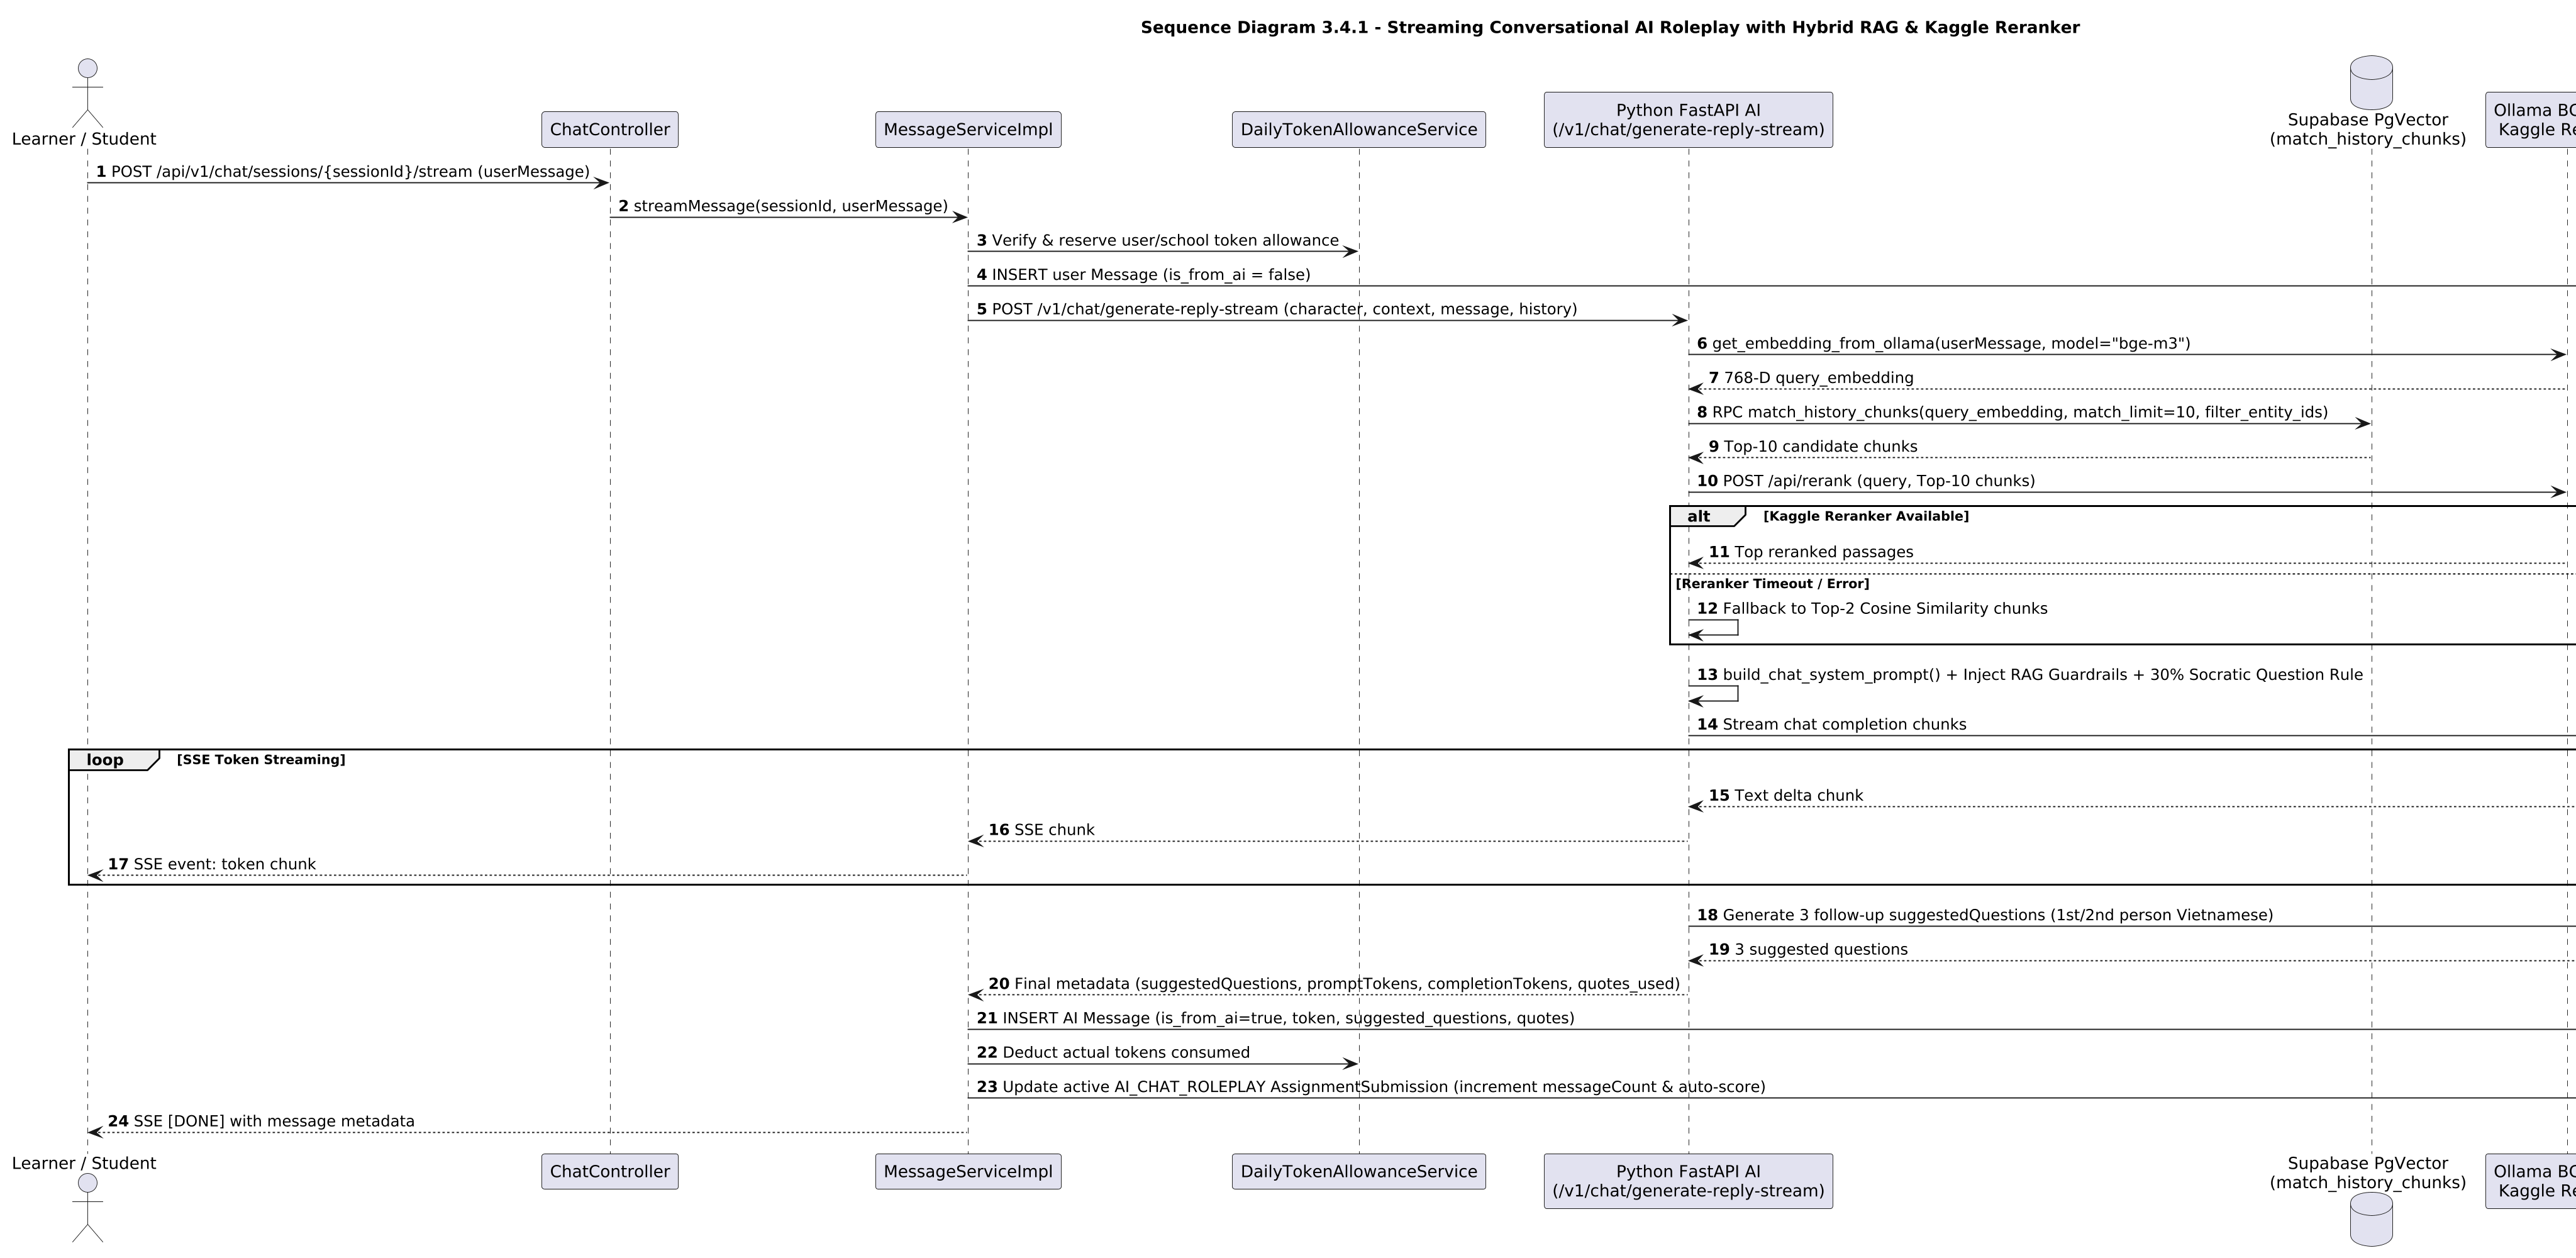
\includegraphics[width=0.98\textwidth]{figures/seq_07_ai_roleplay_chat_rag.png}
    \caption{Sequence Diagram -- Streaming Conversational AI Roleplay with Hybrid RAG \& Kaggle Reranker}
    \label{fig:seq_07_ai_roleplay_chat_rag}
\end{figure}

\newpage
\subsection{Quiz Engine, Question Bank \& Classroom Assignments}

\subsubsection{Class Diagram: Quiz Engine, Question Bank \& Classroom Assignments}

\begin{figure}[H]
    \centering
    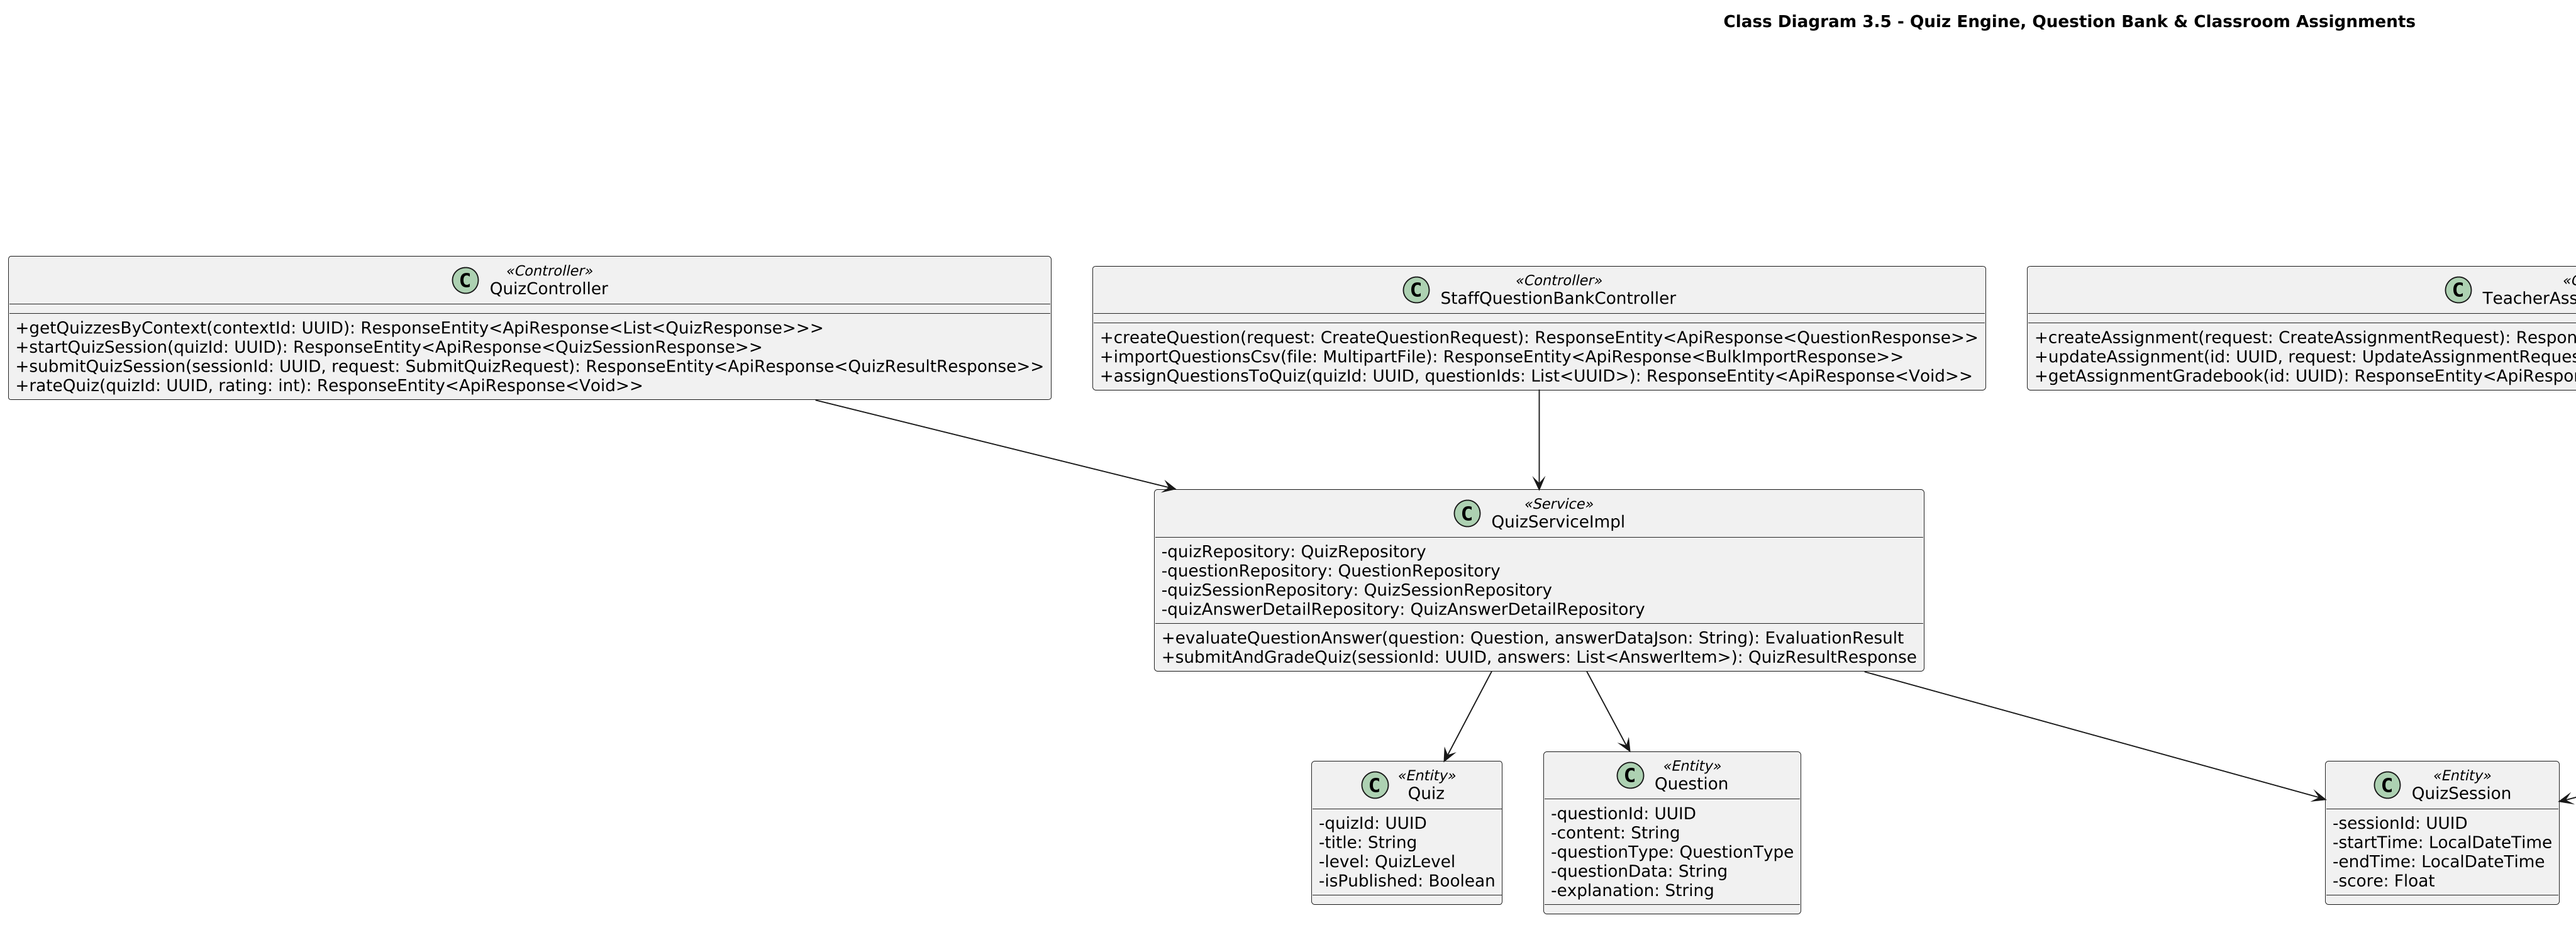
\includegraphics[width=0.98\textwidth]{figures/cls_05_quiz_and_assignment.png}
    \caption{Class Diagram -- Quiz Engine, Question Bank \& Classroom Assignments}
    \label{fig:cls_05_quiz_and_assignment}
\end{figure}

\begin{longtable}{|L{5.5cm}|L{10.0cm}|}
\hline
\rowcolor{tableheader}
\textbf{Class} & \textbf{Description} \\
\hline
\endhead
\texttt{QuizController} / \texttt{StaffQuizController} & REST API controllers managing learner quiz attempts, submissions, ratings, question issue reports, and staff quiz creation/publication. \\
\hline
\texttt{StaffQuestionBankController} & REST API controller (\texttt{/api/v1/staff/question-bank}) supporting polymorphic question creation (\texttt{MULTIPLE\_CHOICE}, \texttt{FILL\_IN\_BLANK}, \texttt{MATCHING}), bulk CSV import, and many-to-many quiz linking. \\
\hline
\texttt{TeacherAssignmentController} & REST API controller (\texttt{/api/v1/teacher/assignments}) enabling teachers to create, update, cancel, or archive classroom assignments and view class gradebooks. \\
\hline
\texttt{StudentAssignmentController} & REST API controller (\texttt{/api/v1/student/assignments}) allowing students to view assigned tasks, start work, log reading duration, and submit completed assignments. \\
\hline
\texttt{QuizServiceImpl} & Evaluates polymorphic JSON question payloads (\texttt{question\_data} vs. \texttt{answer\_data}), computes weighted scores on a 10-point scale, persists \texttt{QuizAnswerDetail} records, and triggers assignment/quest hooks. \\
\hline
\texttt{TeacherAssignmentServiceImpl} / \texttt{StudentAssignmentServiceImpl} & Orchestrates classroom assignment lifecycles, auto-initializes student submission rows, synchronizes AI chat and quiz scores, and classifies on-time (\texttt{SUBMITTED}) vs. late (\texttt{LATE\_SUBMITTED}) completions. \\
\hline
\texttt{Quiz}, \texttt{Question}, \texttt{QuizQuestion}, \texttt{QuizSession}, \texttt{Assignment}, \texttt{AssignmentSubmission} & Domain entities modeling the polymorphic question bank, quiz attempts, classroom assignments, and student gradebook submissions. \\
\hline
\caption{Class Descriptions -- Quiz Engine, Question Bank \& Classroom Assignments}
\label{tab:cls_05_quiz_and_assignment}
\end{longtable}

\subsubsection{Sequence Diagrams: Multi-Type Quiz Grading \& Classroom Assignments}

\begin{figure}[H]
    \centering
    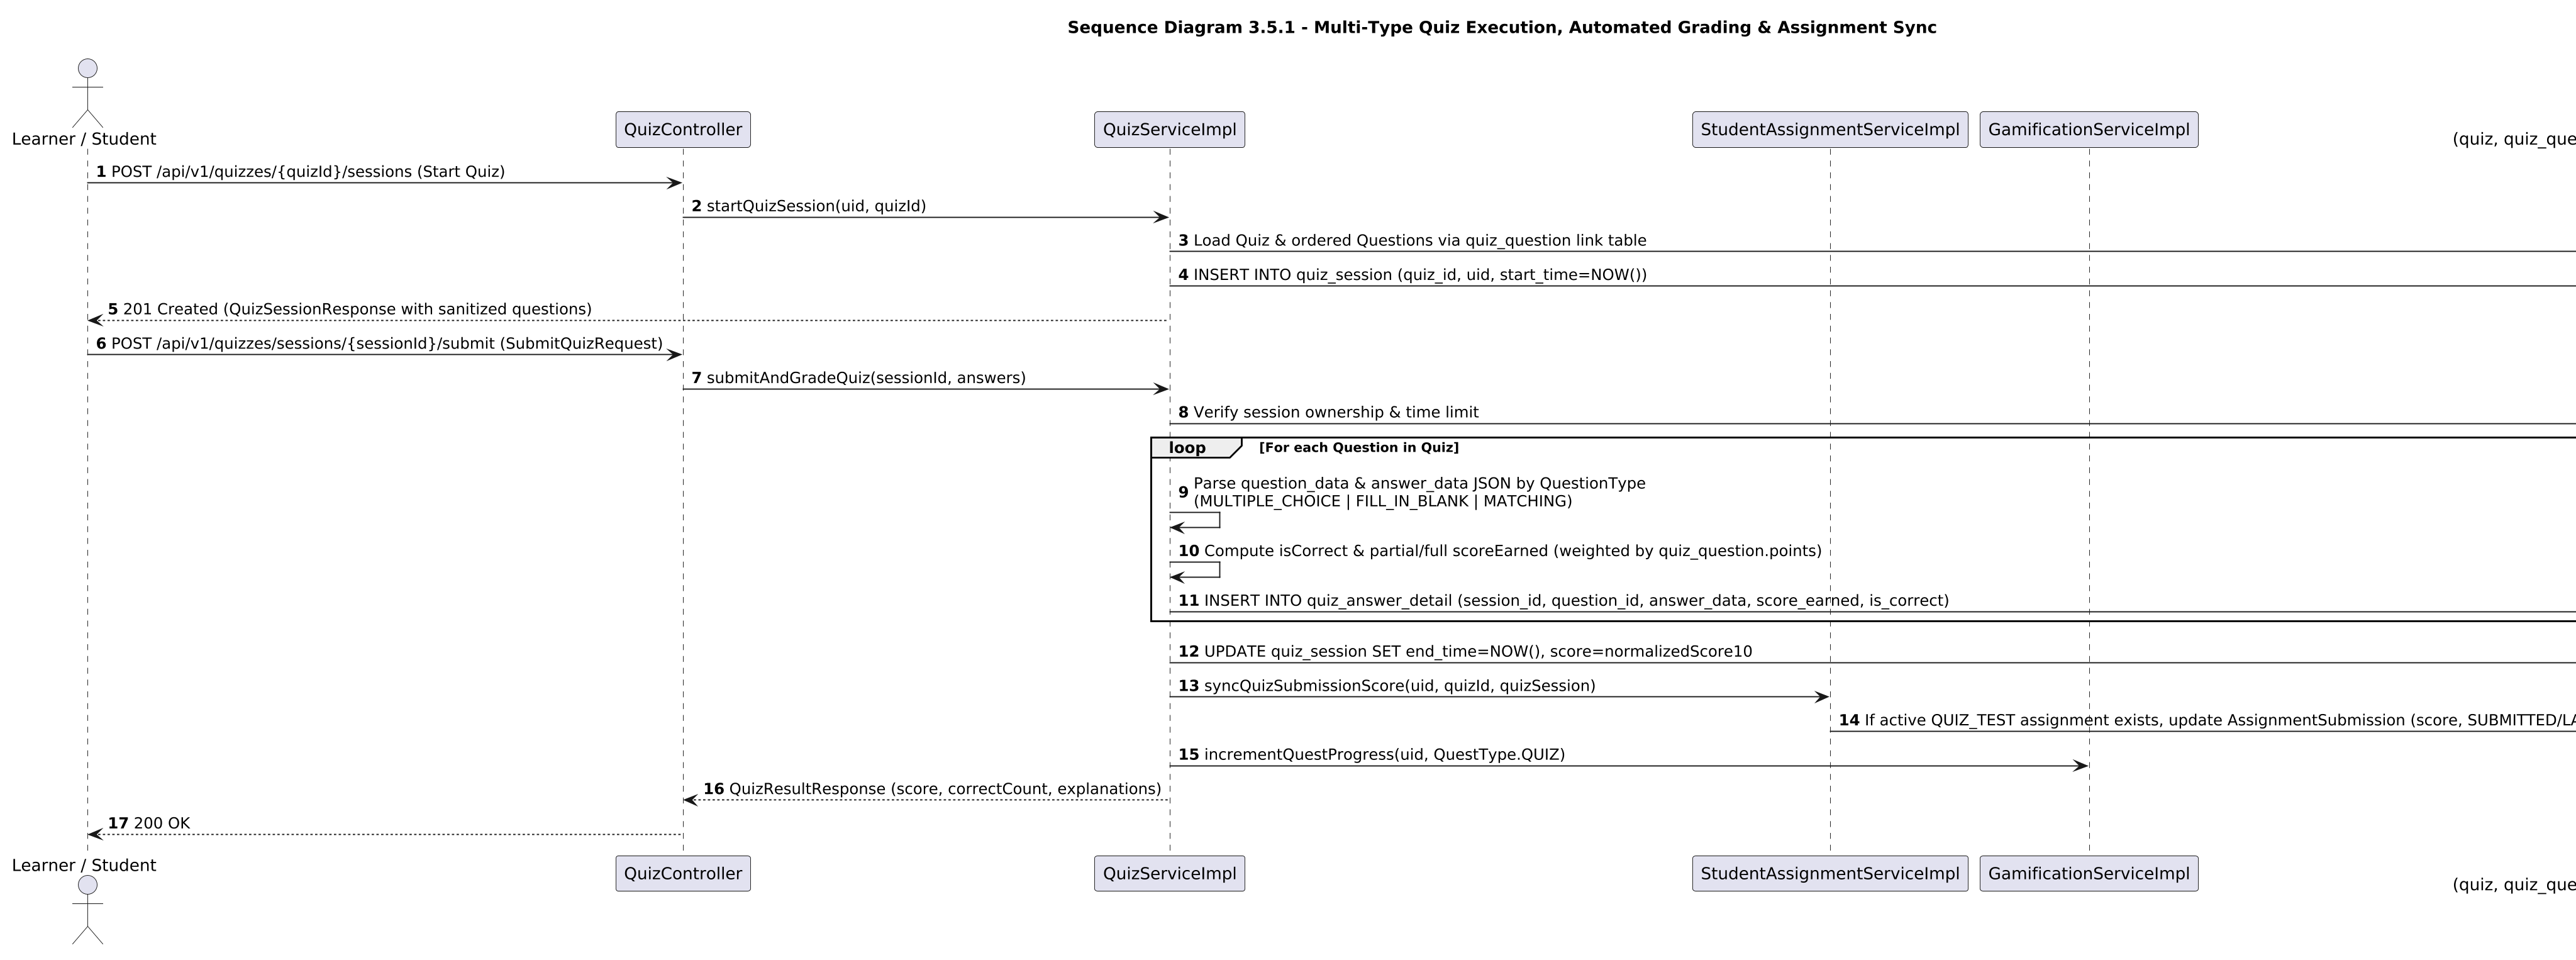
\includegraphics[width=0.98\textwidth]{figures/seq_08_quiz_attempt_and_grading.png}
    \caption{Sequence Diagram -- Multi-Type Quiz Execution, Automated Grading \& Assignment Sync}
    \label{fig:seq_08_quiz_attempt_and_grading}
\end{figure}

\begin{figure}[H]
    \centering
    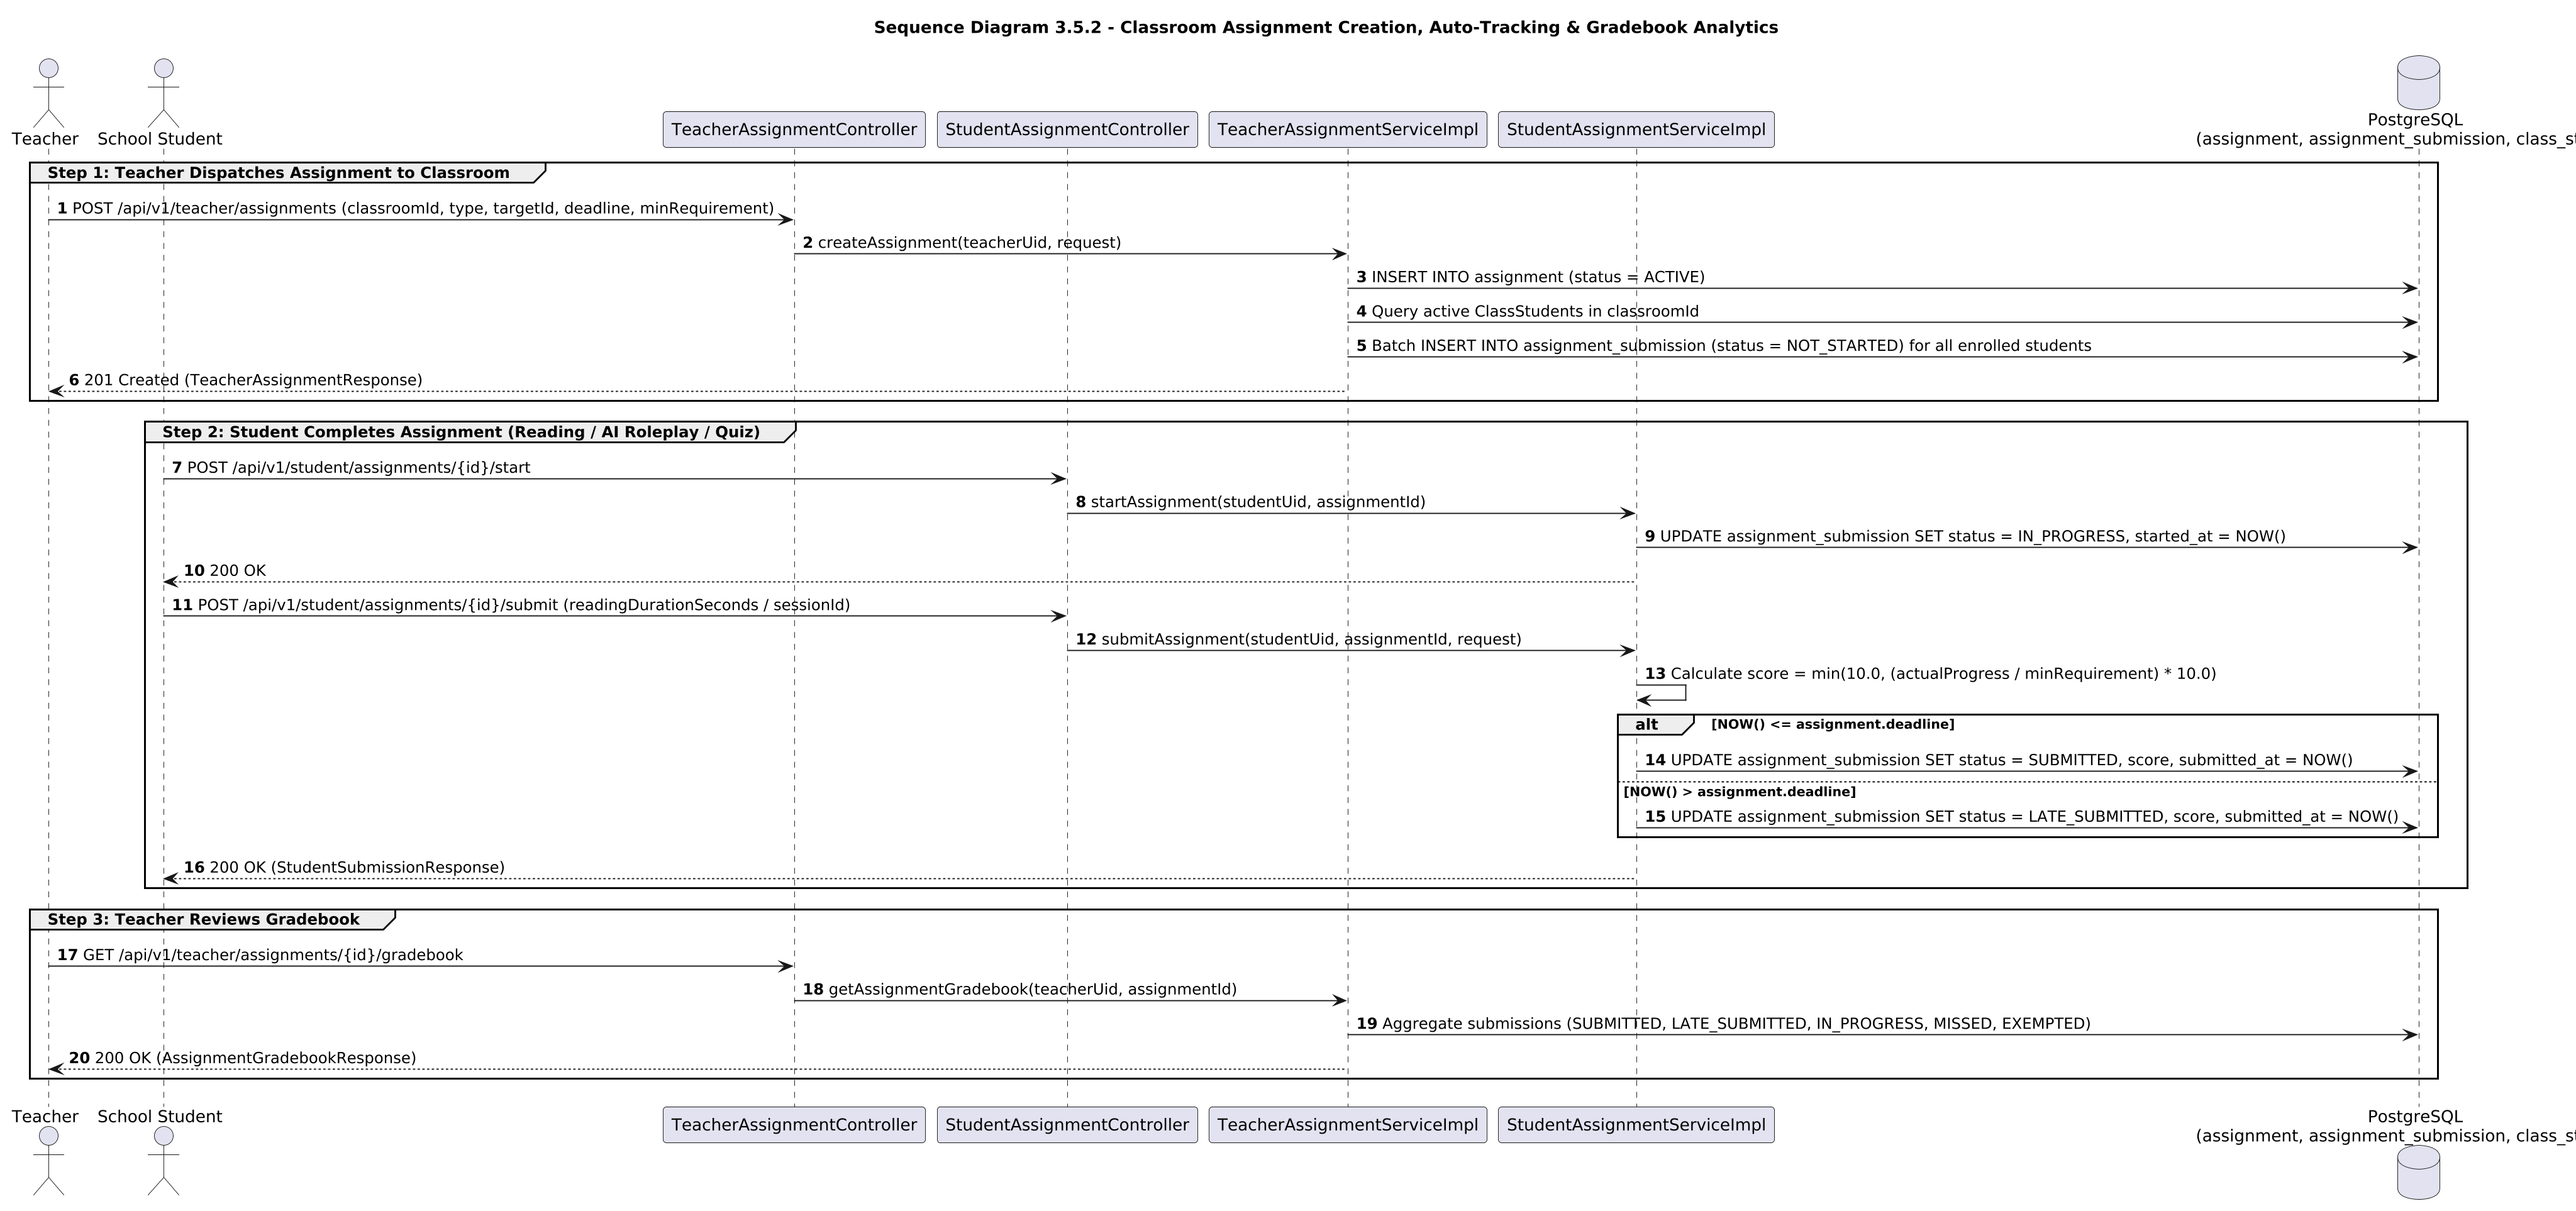
\includegraphics[width=0.98\textwidth]{figures/seq_09_classroom_assignment_submission.png}
    \caption{Sequence Diagram -- Classroom Assignment Creation, Auto-Tracking \& Gradebook Analytics}
    \label{fig:seq_09_classroom_assignment_submission}
\end{figure}

\newpage
\subsection{B2C Subscription, Gamification \& PayOS Payment Fulfillment}

\subsubsection{Class Diagram: B2C Subscription, Gamification \& PayOS Payment Fulfillment}

\begin{figure}[H]
    \centering
    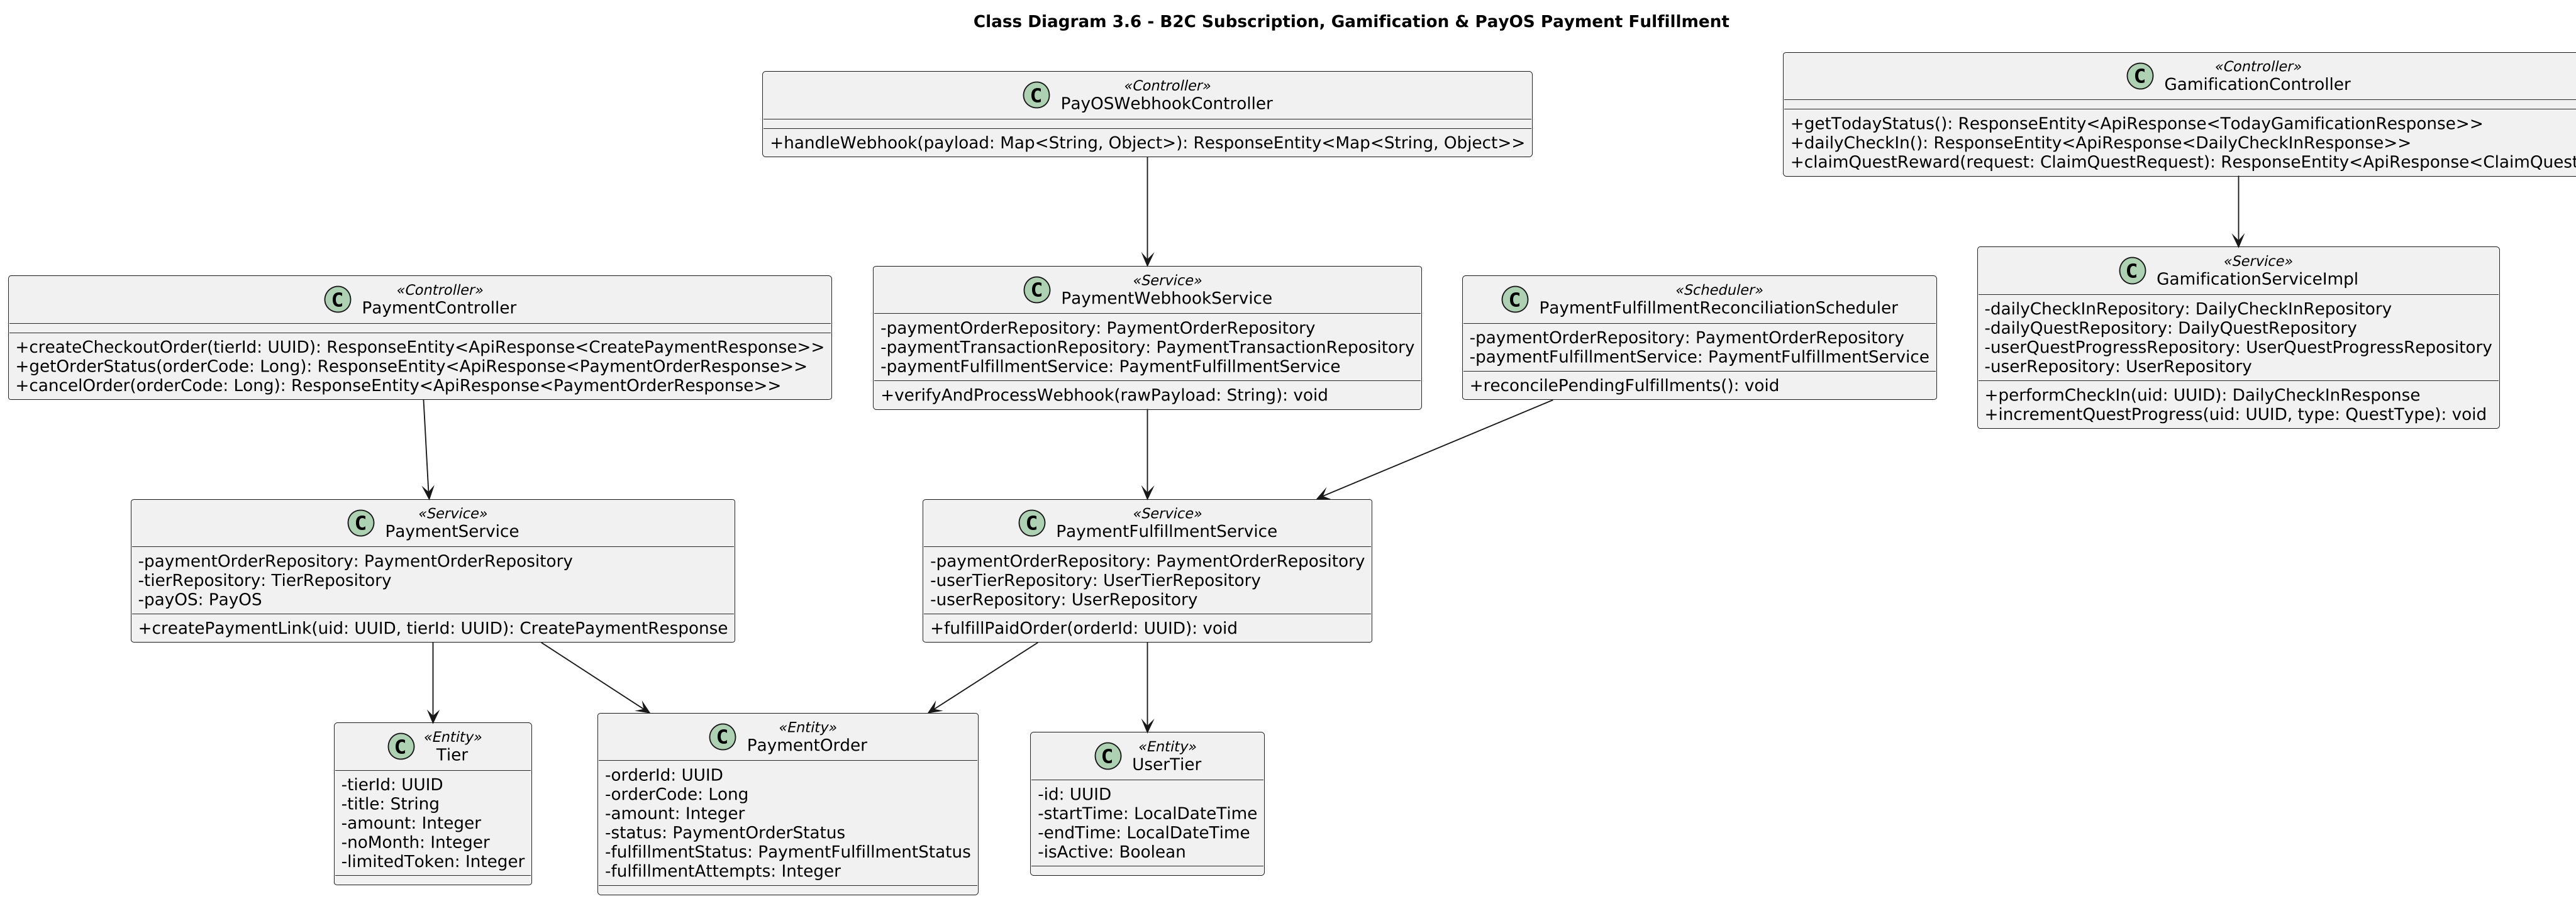
\includegraphics[width=0.98\textwidth]{figures/cls_06_payment_and_gamification.png}
    \caption{Class Diagram -- B2C Subscription, Gamification \& PayOS Payment Fulfillment}
    \label{fig:cls_06_payment_and_gamification}
\end{figure}

\begin{longtable}{|L{5.8cm}|L{9.7cm}|}
\hline
\rowcolor{tableheader}
\textbf{Class} & \textbf{Description} \\
\hline
\endhead
\texttt{PaymentController} & REST API controller (\texttt{/api/v1/payments}) for B2C customers to initiate subscription tier checkouts, poll order status, and cancel pending orders. \\
\hline
\texttt{PayOSWebhookController} & Public webhook endpoint (\texttt{/api/v1/payments/payos/webhook}) receiving asynchronous payment notifications from PayOS. \\
\hline
\texttt{GamificationController} / \texttt{StaffQuestController} & REST API controllers managing daily streak check-ins, daily quest progress queries, token reward claims, and staff quest configurations. \\
\hline
\texttt{PaymentService} / \texttt{PaymentWebhookService} & Generates unique numeric order codes, creates PayOS checkout links, verifies HMAC-SHA256 webhook signatures, and logs immutable \texttt{PaymentTransaction} records. \\
\hline
\texttt{PaymentFulfillmentService} & Executes idempotent, pessimistic-locked order fulfillment (\texttt{PENDING} $\rightarrow$ \texttt{PROCESSING} $\rightarrow$ \texttt{FULFILLED}), activating \texttt{UserTier} and crediting \texttt{Tier.limitedToken} to the user. \\
\hline
\texttt{PaymentFulfillmentReconciliationScheduler} / \texttt{PaymentExpiryScheduler} & Background Spring \texttt{@Scheduled} jobs that retry unfulfilled \texttt{PAID} orders (up to 5 attempts) and transition stale \texttt{PENDING} orders to \texttt{EXPIRED}. \\
\hline
\texttt{GamificationServiceImpl} & Tracks consecutive daily login streaks (\texttt{DailyCheckIn}) and quest progress (\texttt{UserQuestProgress}) across \texttt{CHAT}, \texttt{QUIZ}, and \texttt{READ\_CONTEXT} activities. \\
\hline
\caption{Class Descriptions -- B2C Subscription, Gamification \& PayOS Payment Fulfillment}
\label{tab:cls_06_payment_and_gamification}
\end{longtable}

\subsubsection{Sequence Diagram: PayOS Checkout \& Resilient Tier Fulfillment}

\begin{figure}[H]
    \centering
    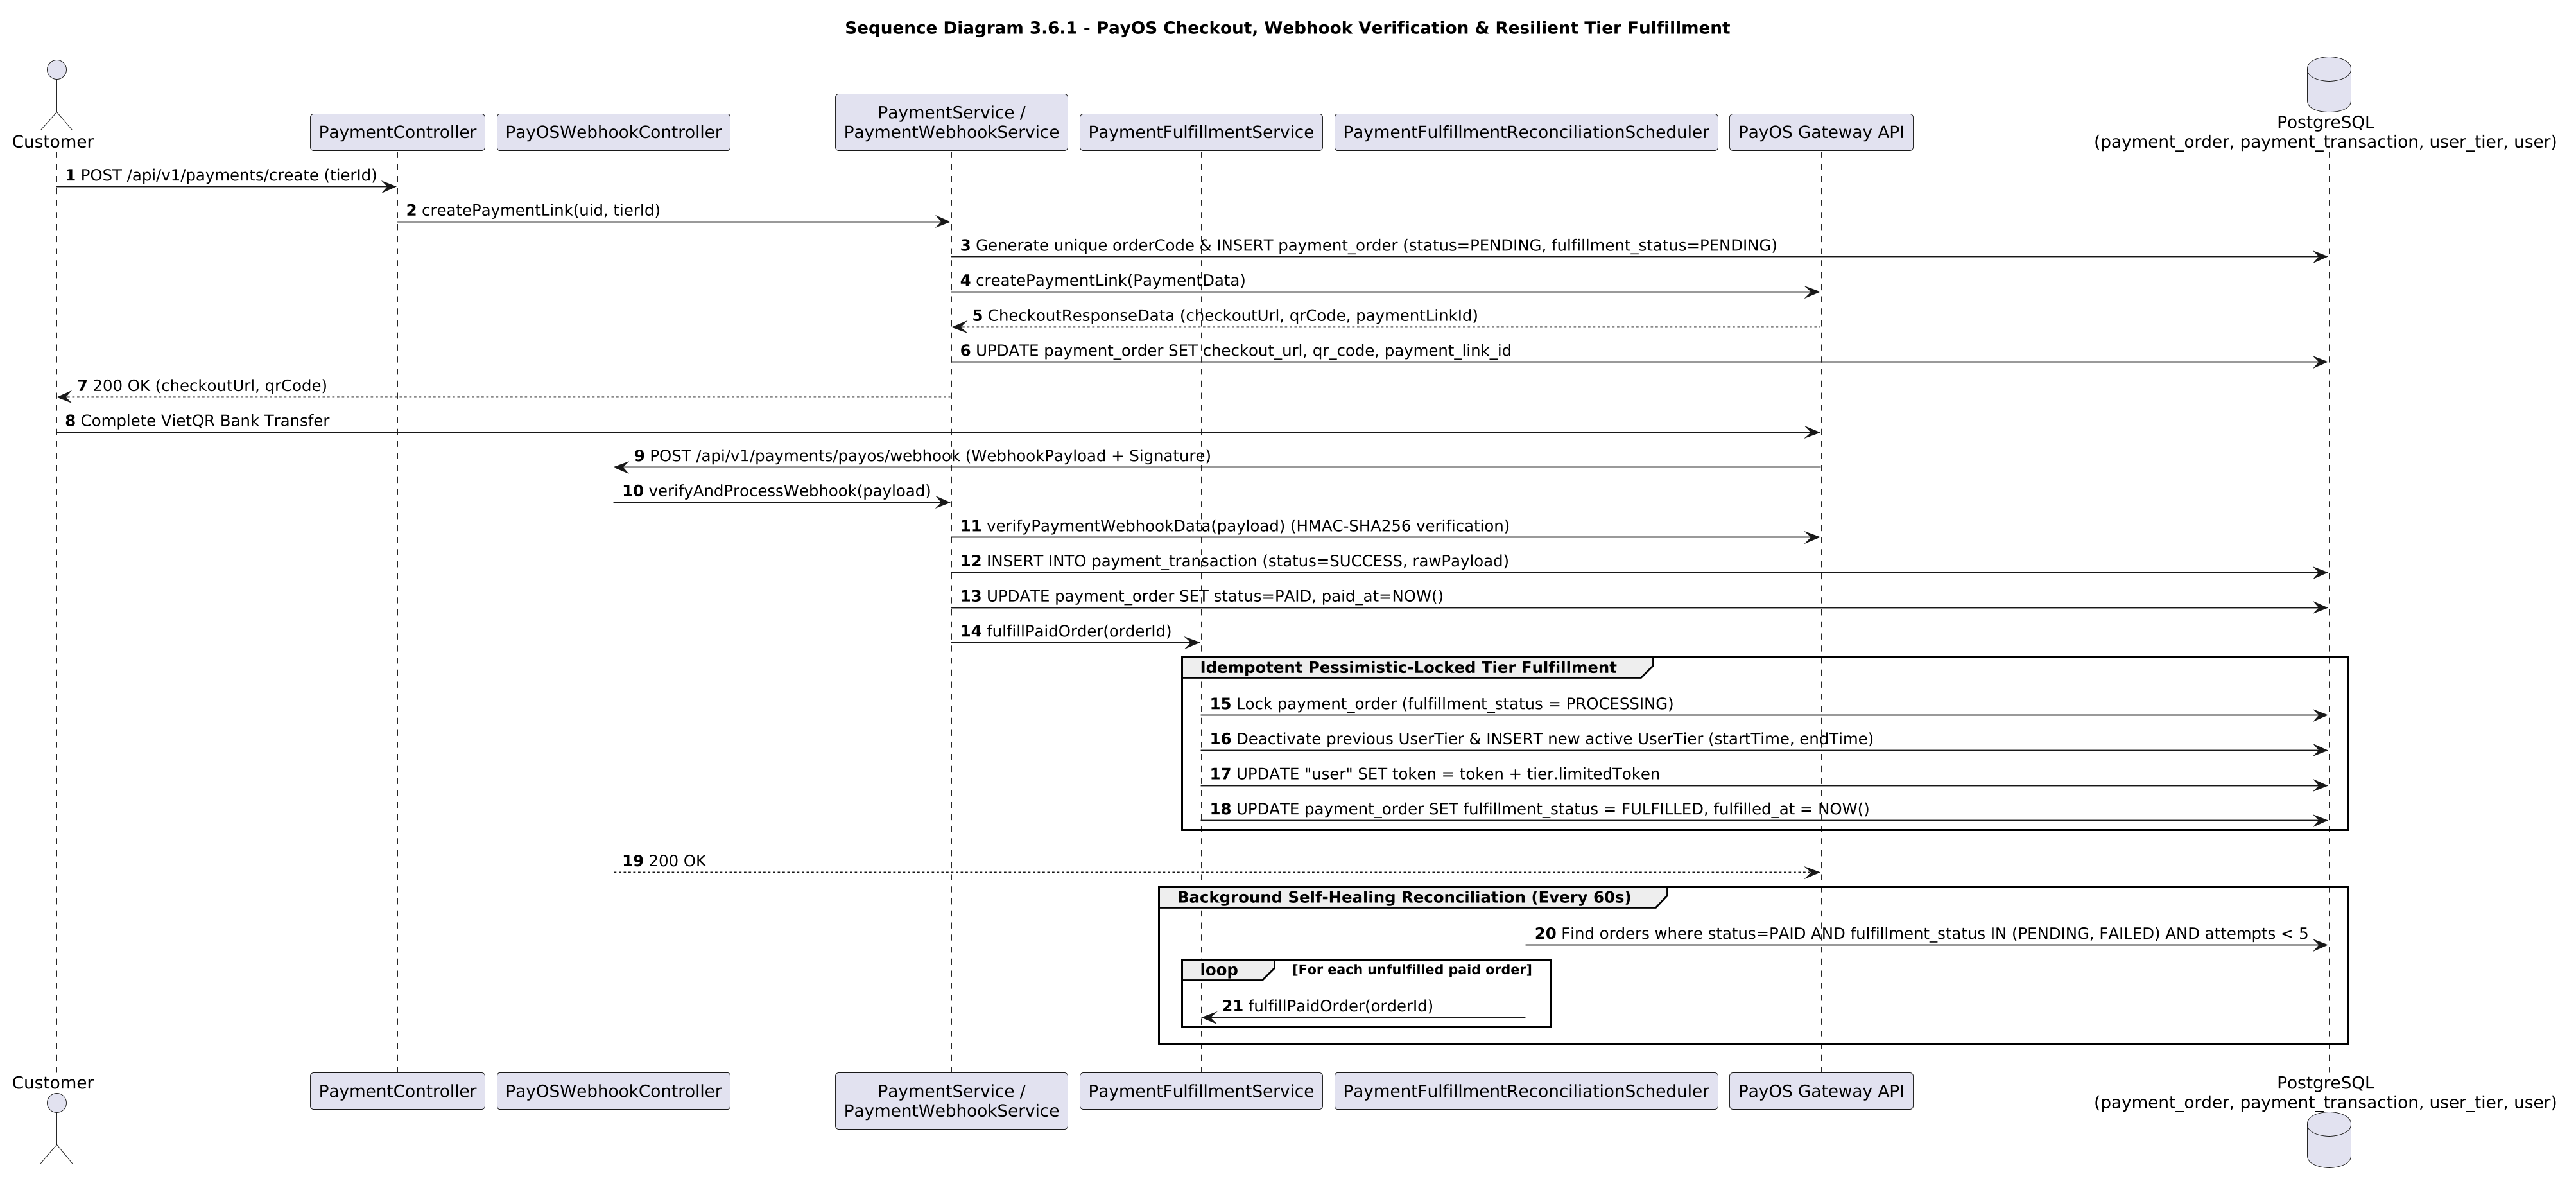
\includegraphics[width=0.98\textwidth]{figures/seq_10_payos_checkout_and_fulfillment.png}
    \caption{Sequence Diagram -- PayOS Checkout, Webhook Verification \& Resilient Tier Fulfillment}
    \label{fig:seq_10_payos_checkout_and_fulfillment}
\end{figure}
